\begin{filecontents}[overwrite]{referencias.bib}
	
	@article{chica2010determinantes,
		author={Chica Gómez, Sandra Milena and Galvis Gutiérrez, Diana Maritza and Ramírez Hassan, Andrés},
		title={Determinantes del rendimiento académico en Colombia. Pruebas ICFES-Saber 11o, 2009},
		journal={Revista Universidad EAFIT},
		volume={46}, number={160}, pages={48--72}, year={2010}
	}
	@article{arria2024estudio,
		author={Buitrago Arria, Daniel and Sánchez Garzón, Laura Camila},
		title={Un estudio de factores socio-económicos asociados al desempeño en el examen Saber 11 en Colombia},
		journal={Maestros \& Pedagogía},
		volume={6}, number={2}, pages={8--31}, year={2024}
	}
	@mastersthesis{lozanofactores,
		author={Lozano Hoyos, Jesús Manuel and Padilla Gamarra, José David and Porto Candamil, Cristian Ángel},
		title={Factores claves que describen los resultados de Pruebas Saber 11 en el departamento del Atlántico usando técnicas de analítica de datos},
		school={Universidad del Norte}, address={Barranquilla, Colombia}, year={2022}, type={Tesis de Maestría}
	}
	@article{miranda2018ingreso,
		author={Miranda, Juan Carlos and Chadid, Yaber and Quintero, Franklin},
		title={Ingreso, clases sociales y Desigualdad educativa en Barranquilla: Colombia},
		journal={Ad-gnosis}, volume={7}, number={7}, pages={8}, year={2018}
	}
	@techreport{icfes2024_informeSaber11_2023,
		author={{Icfes}},
		title={Informe nacional de resultados del examen Saber 11 2023},
		institution={Instituto Colombiano para la Evaluación de la Educación (Icfes)},
		address={Bogotá, Colombia}, year={2024}, month=may,
		url={https://www.icfes.gov.co/wp-content/uploads/2025/04/Informe_Saber11_2023.pdf}
	}
	@article{sanchez2011etnia,
		author={Sánchez Jabba, Andrés},
		title={Etnia y desempeño académico en Colombia},
		journal={Documentos de Trabajo Sobre Economía Regional y Urbana; No. 156}, year={2011}
	}
	@mastersthesis{garcia2012factores,
		author={Corsi García, Luisa Josefa and García Buitrago, María Constanza and Jiménez Archila, Marcela and Niño Garzón, Jeny Paola},
		title={Factores asociados a desempeños destacados y no destacados en las pruebas Saber 11 (2009-2)},
		school={Pontificia Universidad Javeriana}, address={Bogotá, Colombia}, year={2012}, type={Tesis de Maestría}
	}
	@article{garcia2021pruebas,
		author={García Arango, David Alberto and Mejía Cardona, Marco Aurelio and Henao Villa, César Felipe},
		title={Pruebas Saber Pro y Saber 11: análisis de correlaciones aplicado a programas de ingeniería},
		journal={Asociación Colombiana de Facultades de Ingeniería (ACOFI Papers)},
		year={2021}, pages={1--10}
	}
	@mastersthesis{mendieta2024modelo,
		author={Mendieta López, Javier Andrés},
		title={Modelo descriptivo y predictivo para optimizar la mejora en pruebas Saber Pro: un enfoque basado en datos históricos y caracterización estudiantil},
		school={Universidad de Bogotá Jorge Tadeo Lozano}, address={Bogotá, Colombia},
		year={2024}, type={Tesis de Maestría}
	}
	@mastersthesis{granados2025modelado,
		author={Granados López, Hedilberto},
		title={Modelado del desempeño en competencias pruebas Saber Pro: un enfoque multinomial},
		school={Universidad Católica de Manizales}, address={Manizales, Colombia},
		year={2025}, type={Tesis de Maestría}
	}
	@book{tobon2013formacion,
		author={Tobón Tobón, Sergio},
		title={Formación integral y competencias: pensamiento complejo, currículo, didáctica y evaluación},
		publisher={Ecoe ediciones}, address={Bogotá, Colombia}, year={2013}
	}
	@book{cobo2011aprendizaje,
		author={Cobo Romaní, Cristóbal and Moravec, John W},
		title={Aprendizaje invisible. Hacia una nueva ecología de la educación},
		publisher={Publicacions i Edicions Universitat de Barcelona}, year={2011}
	}
	@misc{sapiencia2022_infographicBestSaberPro,
		author={{Icfes and Sapiencia}},
		title={Infographic Best Saber Pro},
		howpublished={Infografía en línea}, year={2022},
		url={https://sapiencia.gov.co/wp-content/uploads/2022/12/infographic-best-saber-pro_anonymous.pdf}
	}
	@mastersthesis{maestre2022_valorAgregadoCalidadEducativa,
		author={Maestre Delgado, Marisol},
		title={El valor agregado como medida de la calidad educativa en instituciones de educación superior en Colombia},
		school={Universidad del Norte}, address={Barranquilla, Colombia},
		year={2022}, type={Tesis de maestría},
		url={https://manglar.uninorte.edu.co/handle/10584/11012}
	}
	@article{vanegas2022_prediccionSaberPro,
		author={Vanegas Ayala, Sebastian Camilo and Leal Lara, Daniel David and Barón Velandia, Julio},
		title={Predicción rendimiento estudiantes pruebas Saber Pro en pandemia junto con las características socioeconómicas},
		journal={Tecnología, Investigación y Academia (TIA)},
		volume={9}, number={2}, pages={5--16}, year={2022}, month=jun, issn={2344-8288}
	}
	@misc{google2025linear,
		author={{Google Developers}},
		title={Linear Regression | Machine Learning Crash Course},
		howpublished={Google Developers}, year={2025}, month=aug,
		url={https://developers.google.com/machine-learning/crash-course/linear-regression}
	}
	@article{mienye2023survey,
		author={Mienye, I. Domor and Jere, N.},
		title={A Survey of Decision Trees: Concepts, Algorithms and Applications},
		journal={IEEE Access}, volume={11}, pages={120192--120208}, year={2023}
	}
	@article{bhatia2010survey,
		author={Bhatia, Neeraj and Kumar, Vandana},
		title={Survey of Nearest Neighbor Techniques},
		journal={arXiv preprint arXiv:1007.0085}, year={2010}
	}
	@article{hodson2022rmse,
		author={Hodson, Tobias O.},
		title={Root-mean-square error (RMSE) or mean absolute error (MAE): when to use them or not},
		journal={Geoscientific Model Development}, volume={15}, pages={5481--5487}, year={2022},
		doi={10.5194/gmd-15-5481-2022}
	}
	@article{chicco2021r2,
		author={Chicco, Javier and Jurman, Giovanni},
		title={The coefficient of determination R-squared is more informative than SMAPE, MAE, MAPE, MSE and RMSE in regression analysis evaluation},
		journal={PeerJ Computer Science}, year={2021}
	}
	@book{han2022data,
		author={Han, Jiawei and Kamber, Micheline and Pei, Jian},
		title={Data Mining: Concepts and Techniques},
		edition={4th}, publisher={Elsevier}, year={2022}
	}
	@article{ozyurt2023educational,
		author={Özyurt, Özcan and Özyurt, Hacer and Mishra, Deepak},
		title={Uncovering the Educational Data Mining Landscape and Future Perspective: A Comprehensive Analysis},
		journal={IEEE Access}, volume={11}, pages={120192--120208}, year={2023}
	}
	@article{alamri2021explainable,
		author={Alamri, Reem and Alharbi, Bandar},
		title={Explainable Student Performance Prediction Models: A Systematic Review},
		journal={IEEE Access}, volume={9}, pages={33132--33143}, year={2021}
	}
	@mastersthesis{cervera2021modelo,
		author={Martínez Cervera, Daniel Esteban},
		title={Modelo de pronóstico en la educación superior en pruebas específicas de ingeniería, licenciatura y pensamiento científico matemático en Saber Pro aplicando Machine Learning},
		school={Universidad Distrital Francisco José de Caldas}, address={Bogotá, Colombia},
		year={2021}, type={Tesis de Maestría}
	}
	@article{del2022indice,
		author={Ramírez del Río, Délany and Guerrero Erazo, Jhonniers},
		title={Índice de desempeño relativo pruebas Saber 11--Saber Pro},
		journal={Encuentro Internacional de Educación en Ingeniería}, year={2022}
	}
	@article{bandura1977self,
		title={Self-efficacy: toward a unifying theory of behavioral change},
		author={Bandura, Albert},
		journal={Psychological review},
		volume={84},
		number={2},
		pages={191},
		year={1977},
		publisher={American Psychological Association}
	}
	@book{vygotsky1978mind,
		title={Mind in society: Development of higher psychological processes},
		author={Cole, Michael},
		year={1978},
		publisher={Harvard university press}
	}
	@article{hanushek1971teacher,
		title={Teacher characteristics and gains in student achievement: Estimation using micro data},
		author={Hanushek, Eric},
		journal={The American Economic Review},
		volume={61},
		number={2},
		pages={280--288},
		year={1971},
		publisher={JSTOR}
	}
	@techreport{icfes2021valoragregado,
		author      = {{Instituto Colombiano para la Evaluación de la Educación (ICFES)}},
		title       = {Medición de los efectos de la educación superior en {Colombia} sobre el aprendizaje estudiantil: Informe técnico},
		institution = {Instituto Colombiano para la Evaluación de la Educación (ICFES)},
		address     = {Bogotá D.C., Colombia},
		month       = apr,
		year        = {2021},
		url         = {https://www.icfes.gov.co/wp-content/uploads/2024/11/Informe-tecnico-1.pdf},
		note        = {[En línea; accedido jun. 2026]}
	}
	@article{bogoya2013modelo,
		title={Un modelo matem{\'a}tico para el valor acad{\'e}mico agregado: Caso de la educaci{\'o}n superior en Colombia},
		author={Bogoya, JD and Bogoya, JM},
		journal={Ingenier{\'\i}a e Investigaci{\'o}n},
		volume={33},
		number={2},
		pages={76--81},
		year={2013}
	}
	@article{bogoya2017value,
		title={Value-added in higher education: ordinary least squares and quantile regression for a Colombian case},
		author={Bogoya, Jose D and Bogoya, Johan M and Pe{\~n}uela, Alfonso J},
		journal={Ingenier{\'\i}a e Investigaci{\'o}n},
		volume={37},
		number={3},
		pages={30--36},
		year={2017},
		publisher={Facultad de Ingenier{\'\i}a, Universidad Nacional de Colombia.}
	}
	@article{rodriguez2022valor,
		title={Valor agregado y las competencias gen{\'e}ricas de los estudiantes de educaci{\'o}n superior en Colombia},
		author={Rodr{\'\i}guez-Revilla, Ramiro and Vallejo-Molina, Rub{\'e}n-Dar{\'\i}o},
		journal={Revista iberoamericana de educaci{\'o}n superior},
		volume={13},
		number={36},
		pages={44--62},
		year={2022},
		publisher={Universidad Nacional Aut{\'o}noma de M{\'e}xico, Instituto de Investigaciones sobre~…}
	}
	@article{mendoza2026valor,
		title={Valor agregado en la educaci{\'o}n superior colombiana: una revisi{\'o}n de la contribuci{\'o}n de los programas y las instituciones a la calidad educativa},
		author={Mendoza-Lozano, Frederick Andr{\'e}s and Pico-Bonilla, Claudia Milena and Bacca-Morales, David and Cano-Ni{\~n}o, Mauricio Alejandro},
		journal={Revista colombiana de educaci{\'o}n},
		number={99},
		year={2026}
	}
	@article{gil2021prediccion,
		title={Predicci{\'o}n del rendimiento acad{\'e}mico estudiantil con redes neuronales artificiales},
		author={Gil-Vera, V{\'\i}ctor D and Quintero-L{\'o}pez, Catalina},
		journal={Informaci{\'o}n tecnol{\'o}gica},
		volume={32},
		number={6},
		pages={221--228},
		year={2021},
		publisher={SciELO Chile}
	}
	@article{garcia2019extraccion,
		title={Extracci{\'o}n de Conocimiento para la Predicci{\'o}n y An{\'a}lisis de los Resultados de la Prueba de Calidad de la Educaci{\'o}n Superior en Colombia},
		author={Garc{\'\i}a-Gonz{\'a}lez, Jos{\'e} R and S{\'a}nchez-S{\'a}nchez, Paola A and Orozco, Manuel and Obredor, Sergio},
		journal={Formaci{\'o}n universitaria},
		volume={12},
		number={4},
		pages={55--62},
		year={2019},
		publisher={SciELO Chile}
	}
	@book{goodfellow2016deep,
		title={Deep learning},
		author={Goodfellow, Ian and Bengio, Yoshua and Courville, Aaron and Bengio, Yoshua},
		volume={1},
		number={2},
		year={2016},
		publisher={MIT press Cambridge}
	}
	@inproceedings{mcqueen1967some,
		title={Some methods of classification and analysis of multivariate observations},
		author={McQueen, James B},
		booktitle={Proc. of 5th Berkeley Symposium on Math. Stat. and Prob.},
		pages={281--297},
		year={1967}
	}
	@article{gil2014analisis,
		title={An{\'a}lisis del procesamiento de los datos de entrada para un localizador de fallas en sistemas de distribuci{\'o}n},
		author={Gil Gonz{\'a}lez, Walter Juli{\'a}n and Mora Fl{\'o}rez, Juan Jos{\'e} and P{\'e}rez Londo{\~n}o, Sandra Milena},
		journal={Tecnura},
		volume={18},
		number={41},
		pages={64--75},
		year={2014},
		publisher={Universidad Distrital Francisco Jos{\'e} de Caldas}
	}
	@techreport{MEN_SINEB_Aprendizaje2023,
		author       = {{Ministerio de Educación Nacional}},
		title        = {Indicadores de aprendizaje: Estadísticas e indicadores
			de educación preescolar, básica y media},
		institution  = {Portal SINEB, Oficina Asesora de Planeación y Finanzas,
			Ministerio de Educación Nacional},
		address      = {Bogotá, Colombia},
		year         = {2023},
		type         = {Ficha de indicadores},
		url          = {https://portalsineb.mineducacion.gov.co/1782/articles-412165_aprendizaje_00_2023.pdf},
		urldate      = {2025-06-27},
		note         = {Sistema de Información Nacional de Educación Básica y Media (SINEB)}
	}
	@techreport{ICFES_FichaMetodologica2022,
		author       = {{Instituto Colombiano para la Evaluación de la Educación}},
		title        = {Ficha metodológica de la operación estadística:
			Medición de la Calidad de la Educación a partir
			de los exámenes {Saber} ({MCEAES})},
		institution  = {Subdirección de Estadísticas, ICFES},
		address      = {Bogotá, Colombia},
		year         = {2022},
		month        = aug,
		type         = {Documento metodológico},
		number       = {PYC-GU009, Versión 002},
		url          = {https://www.icfes.gov.co/wp-content/uploads/2024/11/FICHA_METODOLOGICA_OE.pdf},
		urldate      = {2025-06-27}
	}
	@inproceedings{verleysen2005curse,
		title={The curse of dimensionality in data mining and time series prediction},
		author={Verleysen, Michel and Fran{\c{c}}ois, Damien},
		booktitle={International work-conference on artificial neural networks},
		pages={758--770},
		year={2005},
		organization={Springer}
	}
	
\end{filecontents}

\documentclass[12pt]{article} 

\usepackage{booktabs}
\usepackage{array}
\usepackage{tabularx}
\usepackage{caption}
\usepackage{makecell}
\usepackage{adjustbox}

\usepackage{graphicx}

\usepackage[letterpaper, margin=2.5cm]{geometry}
\usepackage[linktoc=all]{hyperref}
\usepackage{fontspec}
\setmainfont{Times New Roman}
\setlength{\parindent}{1.2cm}

\tolerance=1000
\emergencystretch=\maxdimen
\hyphenpenalty=10000
\hbadness=10000

\usepackage{setspace}                
\onehalfspacing                      

\usepackage{enumitem}                       
\setlist[itemize]{leftmargin=*}      

\usepackage[style=ieee, sorting=none]{biblatex}
\addbibresource{referencias.bib}

\usepackage{url}
\urlstyle{same}

\renewbibmacro*{date}{%
	\iffieldundef{year}
	{\bibstring{nodate}}
	{\printdate}}

\DeclareFieldFormat{url}{[Internet]\adddot\space\bibstring{urlfrom}\space\url{#1}}
\DeclareFieldFormat{urldate}{\adddot\addspace[\bibstring{urlseen}\addcolon\space #1]}

\renewcommand*{\newunitpunct}{\addcomma\space}

\DefineBibliographyStrings{spanish}{%
	urlfrom = {Disponible en},
	urlseen = {Consultado}
} 

\newbibmacro*{author+title+date}{%
	\ifnameundef{editor}
	{}
	{%
		\usebibmacro{editor}%
		\setunit{\addspace}%
		\printnames[byeditor]{editor}%
		\clearname{editor}%
		\newunit
	}%
	\usebibmacro{byeditorx}%
	\usebibmacro{bytranslator+others}%
	\ifnameundef{author}
	{%
		\printfield{title}
		\printtext[parens]{\usebibmacro{date}}
	}%
	{%
		\usebibmacro{author}\addcomma\space%
		\printtext[parens]{\usebibmacro{date}} \adddot \addspace %
		\printfield{title} \adddot
	}%
}

\DeclareBibliographyDriver{online}{%
	\usebibmacro{bibindex}%
	\usebibmacro{begentry}%
	\usebibmacro{author+title+date}%
	\setunit{\adddot\addspace}%
	\printlist{language}%
	\setunit{\adddot\addspace}%
	\usebibmacro{byauthor}%
	\setunit{\adddot\addspace}%
	\usebibmacro{byeditor+others}%
	\setunit{\adddot\addspace}%
	\printfield{version}%
	\setunit{\adddot\addspace}%
	\printfield{note}%
	\newunit\newblock
	\printlist{organization}%
	\setunit{\adddot\addspace}%
	\iftoggle{bbx:eprint}
	{\usebibmacro{eprint}}
	{}%
	\setunit{\adddot\addspace}%
	\usebibmacro{url+urldate}%
	\setunit{\adddot\addspace}%
	\usebibmacro{addendum+pubstate}%
	\setunit{\bibpagerefpunct}\newblock
	\usebibmacro{pageref}%
	\newunit\newblock
	\iftoggle{bbx:related}
	{\usebibmacro{related:init}%
		\usebibmacro{related}}
	{}%
	\usebibmacro{finentry}}

\input{template/packages.tex}
\input{template/toc}
\input{template/sections_config.tex}
\input{template/config} 
\input{template/celdas.tex}
\newcommand{\autoresportada}{
Jostin Alejandro Gómez Restrepo \\
Samuel Giraldo Duque 
}

\newcommand{\autorescitacion}{
J. Gómez Restrepo \\ 
S. Giraldo Duque
}

\newcommand{\autorescitaciontexto}{
Gonzáles Mejía et al
}

\newcommand{\titulo}{Desarrollo de un sistema de información para el análisis comparativo y predictivo de la evolución de competencias académicas entre las pruebas Saber 11 y Saber Pro de los estudiantes de la Universidad San Buenaventura
}

\newcommand{\tituloencabezado}{Desarrollo de un sistema de información para el análisis comparativo y predictivo de la evolución de competencias académicas entre las pruebas Saber 11 y Saber Pro de los estudiantes de la Universidad San Buenaventura}

\newcommand{\tipodocumento}{
Trabajo de Grado presentado
%Anteproyecto presentado
}

\newcommand{\tituloporoptar}{
Ing. Datos y software
%Administrador de empresas
}

%%%%%%%%%%%%%%%%%%%%%%%%%%%%%%%%%%%%%%%
%           Asesor o asesores 
%%%%%%%%%%%%%%%%%%%%%%%%%%%%%%%%%%%%%%%

% si es un solo asesor cambielo a Asesor
\newcommand{\asesorpalabra}{Asesor}

\newcommand{\asesor}{
Jairo Ivan Coy Coy \\
% Doctor(PhD) 
% Especialista(Esp)
% Magíster(MSc)
% Administrador de empresas
}


\newcommand{\grado}{
Trabajo de grado profesional
}

\newcommand{\facultad}{
Facultad de Ingenierías (Bello)
}

\newcommand{\programa}{
Ingeniería Datos y software
}

\newcommand{\sede}{
Bello, Colombia
}

\newcommand{\anio}{
2026
}


\newcommand{\textoconvenio}{

%Posgrados. Si alguna institución en convenio no se encuentra en el listado, ingrésala de forma manual.
%Si no es en convenio o es pregrado, elimina esta línea.
\noindent En convenio con la Universidad (nombre y logo  pequeño de la institución).

%Posgrados. Selecciona cohorte en número romano. Si es pregrado elimina esta línea.
\noindent Seleccione posgrado USB Colombia (A-Z), Cohorte X.

%Los grupos y las líneas de investigación USB Colombia tienen denominaciones predefinidas por la Dirección de Investigaciones. Si algún grupo o línea no se encuentran en el listado, consulta primero con tu asesor o coordinador de investigaciones y luego ingrésalos de forma manual.
\noindent Grupo de Investigación (SIGLA).

\noindent Línea de investigación en.

}



















\begin{document} 
	
	\pagenumbering{arabic}
	
	% Forzar orden de las referencias según el PDF original (1-25)
	\nocite{chica2010determinantes}
	\nocite{arria2024estudio}
	\nocite{lozanofactores}
	\nocite{miranda2018ingreso}
	\nocite{icfes2024_informeSaber11_2023}
	\nocite{sanchez2011etnia}
	\nocite{garcia2012factores}
	\nocite{garcia2021pruebas}
	\nocite{mendieta2024modelo}
	\nocite{granados2025modelado}
	\nocite{tobon2013formacion}
	\nocite{cobo2011aprendizaje}
	\nocite{sapiencia2022_infographicBestSaberPro}
	\nocite{maestre2022_valorAgregadoCalidadEducativa}
	\nocite{vanegas2022_prediccionSaberPro}
	\nocite{google2025linear}
	\nocite{mienye2023survey}
	\nocite{bhatia2010survey}
	\nocite{hodson2022rmse}
	\nocite{chicco2021r2}
	\nocite{han2022data}
	\nocite{ozyurt2023educational}
	\nocite{alamri2021explainable}
	\nocite{cervera2021modelo}
	\nocite{del2022indice}
	
	\renewcommand{\headrulewidth}{1pt}
	\renewcommand{\headrule}{\hbox to\headwidth{%
			\color{orange}\leaders\hrule height \headrulewidth\hfill}}
	
	\definecolor{fgheader}{gray}{.5}
	
	\fancyhead{}
	\fancyhead[L]{\fontsize{10}{12} \selectfont \textcolor{gray}{\tituloencabezado}}
	\fancyhead[R]{\textcolor{gray}\thepage}
	\fancyfoot{}
	\setlength{\headheight}{24.64995pt}
	
	\selectlanguage{english}
	\pagestyle{empty}
	
	\input{templatepages/paginaportada}
	
	\footnotesize
	\input{templatepages/paginalegal}
	\normalsize
	
	
%regresa el valor de 12 pixeles
\normalsize
%\thispagestyle{empty}


\noindent \begin{center}
\textbf{Dedicatoria}
\par\end{center}

 \vspace{0.7mm}
 
 \begin{center}
     A mis padres, Carolina Duque y Andrés Giraldo, por ser el origen de todo lo que soy, aparte de su amor y el apoyo incondicional detrás de cada paso en este camino.
     
     A mi madrastra, Natalia Pérez, por su amor, su dedicación y su constante acompañamiento.
     
     A mi hermano, Matías Giraldo, por ser mi compañero de vida, por su apoyo y por los momentos que compartimos.
     
     A mis abuelos, Edelmira Murcia y Carlos Giraldo, Lucy Torrente y Alberto Duque, y a Patricia Marín, por sembrar en mí, con su ejemplo, el valor del esfuerzo y la constancia.
     
     A mis tías, Alejandra Duque, Martha Duque, Aura María Giraldo y Catalina Ríos, a mis tíos, Alberto Duque, Guillermo Gaviria, Julián Giraldo y Carlos Andrés Pérez, y a mi primo Jacobo Gaviria, por su cariño y por acompañarme siempre.
     
     A mis ahijados, Lucca y Benjamin Gaviria, que Dios les tenga preparada una vida llena de salud y prosperidad.
     
     A mi novia, Nycolle López, por su paciencia, su compañía y su aliento en los momentos más exigentes de este proceso.
     
     A Thomas Grisales, Simón Gaviria, Jacobo Ortiz y Daniel Pulgarin, mis amigos de toda la vida, por su amistad incondicional y por las historias que compartimos.
     
     A Jaime Miranda, Alejandro Vega y Juan José Mesa, amigos de estos últimos años, por su compañía sincera, por los momentos que hemos vivido juntos.
     
     A Jostin Gómez, por ser mi compañero inseparable en esta travesía académica, compartiendo cada aula, cada reto y cada logro que define nuestra formación universitaria.
     
     A todos ellos y a Dios, mi más profunda gratitud. \vspace{0.5cm}
 \end{center}
 
 \begin{flushright}
 	\textbf{Samuel Giraldo Duque}
 \end{flushright}
 
 \newpage
 
 \begin{center}
 	A quienes caminaron conmigo sin saber muy bien hacia dónde, y aun así no se detuvieron.
 	Hay una fuerza que no tiene nombre exacto y que, sin embargo, empuja a las personas a seguir, a preguntar, a no quedarse quietas ante lo desconocido. Esa fuerza —que corre por la sangre antes de tener explicación— fue la misma que me trajo hasta aquí. Ustedes la reconocieron en mí antes que yo, y la alimentaron con paciencia, incluso cuando el camino no tenía todavía forma ni nombre.
 	Esta tesis es, apenas, una de las respuestas posibles a esa pregunta que nunca dejamos de hacernos.
 	A Dios, que ha germinado en mí el don del entendimiento, dándome la fortaleza y la capacidad para seguir adelante.
 	A mi madre, Miryam Restrepo, por su amor incondicional y sostenerme incluso en los días más difíciles.
 	A mi padre, Henry Gómez, por enseñarme a caminar con paso firme y silencioso, y por estar ahí, siempre, aunque no siempre lo dijera con palabras.
 	A mi hermano, Cristian Gómez, mi primer compañero de vida, con quien comparto no solo la sangre sino la historia, las motivaciones, los sueños y las aspiraciones.
 	A mis abuelos maternos, Rocío Giraldo y Jesús Evelio Restrepo, por el cariño y el apoyo que se siente aún en la distancia y en el tiempo.
 	A mis abuelos paternos, María Vitalina Patiño y Miguel Ángel Gómez, quienes aunque la vida no me permitió disfrutarlos por mucho tiempo, dejaron una huella que indiscutiblemente también me formó.
 	A Juan David Quintana y Juan Sebastián Mosos, amigos que convirtieron el camino en algo más liviano de recorrer.
 	A Samuel Giraldo, compañero de tesis y, con el tiempo, algo más que un compañero: gracias por hacer de este proceso algo compartido, y no solo cumplido. \vspace{0.5cm}
 \end{center}
 
 \begin{flushright}
 	\textbf{Jostin Alejandro Gómez Restrepo}
 \end{flushright}


 %\vspace{6.0cm}
 \newpage

\noindent \begin{center} 
 \textbf{Agradecimientos}
\par\end{center}

 \vspace{0.7mm}
 
 \begin{center}
     Agradezco profundamente a mi familia por su apoyo incondicional, a mis amigos por su compañía y motivación constante, y a la Universidad de San Buenaventura por proporcionar los recursos necesarios para desarrollar este trabajo. Un agradecimiento especial al docente Jairo Iván Coy Coy, asesor de esta tesis, cuya guía experta y disponibilidad fueron fundamentales para la realización de este proyecto. \vspace{0.5cm}
 \end{center}
 
 \begin{flushright}
 	\textbf{Samuel Giraldo Duque} \vspace{1cm}
 \end{flushright}
 
 \begin{center}
 	Expreso mi sincero agradecimiento a la Universidad de San Buenaventura, por brindarme la formación académica, los recursos y el espacio necesarios para el desarrollo de este trabajo.
 	Un agradecimiento especial al docente Jairo Iván Coy Coy, asesor de esta tesis, cuya guía no se limitó a lo técnico: su disposición constante, su paciencia y su compromiso genuino con este proyecto marcaron una diferencia real en su desarrollo. Sus aportes y su exigencia fueron determinantes para llevar este trabajo a buen término.
 	Agradezco también a los docentes y funcionarios de la Universidad que, de una u otra forma, contribuyeron con su conocimiento y disposición al desarrollo de este trabajo.
 	A mi familia y amigos, gracias por su respaldo constante a lo largo de este proceso; su apoyo, aliento y comprensión fueron un soporte fundamental para poder cumplir con esta meta.
 	Finalmente, agradezco a todas las personas que, directa o indirectamente, aportaron su tiempo, conocimiento o colaboración para hacer posible este resultado. \vspace{0.5cm}
 \end{center}
 
 \begin{flushright}
 	\textbf{Jostin Alejandro Gómez Restrepo}
 \end{flushright}
 
 

\cleardoublepage{}

	
	\tableofcontents{}
	\cleardoublepage{}
	
	\listoftables
	\cleardoublepage{}
	
	\listoffigures
	
	\clearpage
	\phantomsection
	\addcontentsline{toc}{section}{RESUMEN}
	\section*{RESUMEN}
	\pagestyle{fancy}
	Este trabajo presenta un sistema de información para el análisis comparativo y predictivo de la evolución de competencias académicas entre las pruebas Saber 11 y Saber Pro. Para el desarrollo del estudio se utilizaron cerca de $1,32$ millones de registros de estudiantes emparejados de manera individual. Con esta información se integraron los resultados de ambas pruebas en una base de datos relacional y se diseñó un modelo de valor agregado apoyado en una red neuronal artificial de tipo perceptrón multicapa. Los resultados obtenidos por este modelo se compararon con los realmente alcanzados mediante técnicas de referencia como la regresión lineal y el algoritmo de agrupamiento K-means. El proceso de estimación se realizó bajo dos escenarios diferentes: uno que incluía variables socioeconómicas y otro que no las consideraba. Esta comparación permitió analizar en qué medida los factores de contexto influyen en el desempeño académico de los estudiantes. Los resultados muestran una capacidad explicativa moderada ($R^2$ entre $0,39$ y $0,61$), en la que la red neuronal supera a los modelos de referencia salvo en inglés, y un valor agregado institucional mayoritariamente negativo. Estos hallazgos no confirman la hipótesis inicial, pero el sistema desarrollado cumple su función analítica y se materializa en un tablero interactivo de apoyo a la toma de decisiones institucionales



\palabrasclave{valor agregado educativo, Saber 11, Saber Pro, redes neuronales artificiales, sistema de información} 
	
	\clearpage
	\phantomsection
	\addcontentsline{toc}{section}{ABSTRACT}
	\section*{ABSTRACT}
	This work develops an information system for the comparative and predictive analysis of the evolution of academic competencies between the Saber 11 and Saber Pro tests at Universidad de San Buenaventura. Based on approximately 1.32 million individually matched student pairs, both tests were integrated into a relational database, and a value-added model was built whose predictive engine is an artificial neural network of the multilayer perceptron type, benchmarked against linear regression and K-means segmentation reference models. The estimation was carried out under two input configurations, with and without socioeconomic variables, in order to quantify the contribution of context. The results show a moderate explanatory capacity (R² between 0.39 and 0.61), in which the neural network outperforms the reference models except in English, and a predominantly negative institutional value added. These findings do not confirm the initial hypothesis, yet the developed system fulfills its analytical purpose and materializes in an interactive dashboard supporting institutional decision-making.



\keywords{educational value added, Saber 11, Saber Pro, artificial neural networks, information system}
	
	\setcounter{secnumdepth}{5}  
	
	\section{INTRODUCCIÓN}
	La calidad de la educación superior en Colombia es un tema que ha cobrado cada vez más relevancia tanto para las instituciones educativas como para la comunidad académica, especialmente en lo relacionado con la evaluación del desarrollo de competencias durante la trayectoria formativa de los estudiantes. En este contexto, el Instituto Colombiano para la Evaluación de la Educación (ICFES) aplica dos pruebas estandarizadas de gran importancia: la prueba Saber 11, que se presenta al finalizar la educación media, y la prueba Saber Pro, aplicada al culminar la formación universitaria de pregrado.
Estas evaluaciones permiten analizar el desempeño de los estudiantes en distintos momentos de su proceso educativo y constituyen una valiosa fuente de información para comprender cómo evolucionan sus competencias a lo largo del tiempo. Sin embargo, a pesar del potencial que ofrecen estos datos, pocas instituciones de educación superior los han utilizado de manera sistemática para relacionar los resultados obtenidos al ingreso y al final de la formación universitaria, identificar tendencias de mejora o estancamiento y respaldar decisiones académicas con evidencia objetiva. La Universidad de San Buenaventura también enfrenta este desafío, pero al mismo tiempo cuenta con una oportunidad importante para aprovechar la información histórica disponible y transformarla en conocimiento útil para fortalecer sus procesos académicos y de mejora continua.
Con el propósito de aportar en este sentido, este trabajo desarrolla un sistema de información con capacidades predictivas y comparativas orientado a analizar la evolución de las competencias de los estudiantes entre las pruebas Saber 11 y Saber Pro. Para ello, se integran los resultados de ambas evaluaciones junto con variables contextuales y socioeconómicas relevantes, lo que permite construir modelos estadísticos y de aprendizaje automático capaces de estimar el desempeño esperado de los estudiantes y medir el valor agregado que la institución aporta durante su proceso de formación.
Desde el campo de la ingeniería de datos y bajo este argumento, este proyecto representa una aplicación concreta de técnicas de minería de datos educativos (\textit{Educational Data Mining}, EDM), análisis estadístico, visualización interactiva al ámbito de la gestión académica universitaria y la integración de modelos basados en sistemas inteligentes. El uso de algoritmos como la regresión lineal, los árboles de decisión y el método de los $k$ vecinos más cercanos (KNN) permitirá construir modelos robustos de predicción, mientras que los tableros de control (\textit{dashboards}) facilitarán la interpretación de resultados por parte de los tomadores de decisiones institucionales.

	
	\section{PLANTEAMIENTO DEL PROBLEMA}
	El seguimiento del progreso académico de los estudiantes a lo largo de su formación universitaria constituye una herramienta clave para medir la calidad educativa y orientar estrategias de mejora continua. Sin embargo, existe una oportunidad de mejora basada en los datos que cada universidad recolecta de las pruebas Saber 11 y Saber Pro que no es comúnmente aprovechada, y que consiste en tomar toda esta información y transformarla en decisiones de negocio que se reflejen en mejores resultados académicos en los estudiantes.
Esta situación surge dado que la mayoría de las instituciones de educación superior no disponen de sistemas que integren y analicen de manera estructurada la información proveniente de la prueba Saber Pro y se alíe con instituciones escolares que les proporcione información sobre los resultados de las pruebas Saber 11 recientes. A su vez, esta falta de integración impide realizar análisis comparativos que permitan evaluar la evolución de las competencias adquiridas durante el proceso de formación~\cite{garcia2021pruebas}.
En el caso de la Universidad San Buenaventura, donde todavía se cuenta con esta falencia, se muestra como una oportunidad de mejora, contar con un sistema de información que relacione los resultados de ambas pruebas facilitando la identificación de patrones de aprendizaje, fortalezas institucionales y áreas de oportunidad para cada programa académico~\cite{mendieta2024modelo}. La ausencia de este tipo de herramientas limita la capacidad de realizar predicciones sobre el rendimiento futuro de los estudiantes y restringe la generación de estrategias pedagógicas basadas en evidencia~\cite{icfes2024_informeSaber11_2023}.
Por lo tanto, se presenta la necesidad de desarrollar un sistema que consolide los datos de las pruebas Saber Pro, que incorpore técnicas estadísticas y modelos predictivos permitiendo anticipar la fluctuación de las competencias académicas a lo largo del proceso educativo.



	
	\section{ANTECEDENTES}
	Los factores estructurales y contextuales que tienen incidencia en los puntajes de las pruebas Saber 11 han sido estudiados en la literatura colombiana, lo que permite fundamentar qué información se requiere capturar y a partir de está, generar un sistema de información que busque realizar un análisis comparativo y predictivo con robustez.
Uno de los estudios más citados es el que realizó~\cite{chica2010determinantes}, en el año 2010, donde mediante un modelo Logit Ordenado generalizado se encontraron impactos positivos y significativos de variables como nivel de ingreso del hogar, escolaridad de los padres, tipo de jornada escolar y naturaleza del colegio (oficial vs.\ no oficial) sobre los puntajes en matemáticas y lenguaje. El estudio de~\cite{arria2024estudio}, en el año 2024, encontró que los puntajes bajos se asocian sistemáticamente con carencia de recursos educativos, bajo nivel educativo de los padres y condiciones de vida menos favorables, mientras que los puntajes altos se relacionan con mayores ingresos y mejores entornos familiares.
En el Atlántico, la investigación realizada por~\cite{lozanofactores}, en el año 2022, aplicó análisis demográficos, sociales y económicos para identificar variables determinantes del rendimiento en Saber 11, tales como el acceso a internet, características del colegio y variables socioeconómicas del estudiante. Otro estudio regional, realizado por~\cite{miranda2018ingreso}, en el año 2018, encontró que el ingreso del hogar, el estrato socioeconómico y la educación de los padres tienen efectos estadísticamente significativos sobre el puntaje en Saber 11, y que la educación de los padres contribuye de forma similar y consistente al rendimiento académico del hijo.
Adicionalmente, el informe nacional del ICFES del año 2023,~\cite{icfes2024_informeSaber11_2023}, presenta análisis de efectos marginales en modelos estadísticos que muestran cómo factores económicos, familiares y escolares inciden en los resultados del examen Saber 11 a nivel nacional, incluyendo variables como la condición de población víctima del conflicto armado, lo que permite dimensionar desigualdades territoriales y sociales.
Por su parte,~\cite{sanchez2011etnia} en el año 2011, documenta que los estudiantes pertenecientes a etnias cómo indígena, afrocolombiana, raizal y rom, obtienen en promedio puntajes inferiores, y que aunque parte de esa brecha se explica por características observables (familiares, institucionales y sociales), otra parte se debe a factores no observados, lo que implica que el sistema debe contemplar variables latentes o de contexto para capturar esta variación.
Finalmente, el estudio realizado por~\cite{garcia2012factores}, en el año 2012, estudia múltiples grupos de variables independientes ---demográficas, socioeconómicas, familiares, escolares e institucionales--- y encuentra que la zona y condicion de trabajo, pertenecer a una etnia, la pérdida de grados, el tipo de colegio, la jornada escolar y el acceso a internet son determinantes significativos del desempeño destacado frente al no destacado.
Estos antecedentes muestran que los factores que consistentemente aparecen asociados al rendimiento en Saber 11 incluyen condiciones como el nivel socioeconómico, ingresos económicos del hogar, escolaridad de los padres, tipo de colegio (oficial/privado), jornada escolar, acceso a recursos como internet o computadores, etnia, pérdida de grados, así como diferencias regionales y contextuales.
Para el sistema propuesto, esto implica que debe diseñarse para recolectar, limpiar e integrar estas variables, asegurar que los datos sean representativos (territorialidad, diversidad de programas, etc.) e incorporar métodos de modelado que permitan comparar subgrupos, estimar efectos marginales y posiblemente identificar variables no observadas o proxies (sustitutas) que reflejen el contexto institucional. De esta manera, se podrán lograr predicciones útiles y sobre todo, crear y diseñar estrategias institucionales orientadas a fortalecer las competencias académicas de los estudiantes.
	
	\section{JUSTIFICACIÓN}
	La implementación de un sistema de información con capacidades predictivas y comparativas facilitará el análisis del desempeño académico de los estudiantes y aportará una visión más clara sobre su proceso de formación~\cite{granados2025modelado}. Este proyecto busca integrar los resultados de las pruebas Saber 11 y Saber Pro en una única plataforma de análisis que permita comprender cómo evolucionan las competencias de los estudiantes desde su ingreso a la universidad hasta la finalización de sus estudios. A través de esta herramienta, la Universidad de San Buenaventura podrá identificar patrones de mejora o posibles áreas de estancamiento en el desarrollo de competencias, así como reconocer los factores que tienen mayor influencia en el rendimiento académico. Esta información servirá de apoyo para definir estrategias orientadas al fortalecimiento de la calidad educativa y al mejoramiento continuo de los procesos formativos.
Asimismo, la incorporación de técnicas estadísticas y modelos predictivos permitirá respaldar la toma de decisiones con información objetiva y basada en evidencia~\cite{tobon2013formacion}. Desde una perspectiva académica, el proyecto también aporta una aplicación práctica de la ingeniería de datos en el ámbito educativo, demostrando cómo el análisis de información puede convertirse en una herramienta valiosa para comprender mejor los resultados de aprendizaje y contribuir al fortalecimiento de la educación superior. Este sistema representa un avance significativo hacia la transformación digital en la gestión educativa, permitiendo a la universidad disponer de una plataforma sólida para el monitoreo, análisis y predicción del desempeño de sus estudiantes.


	
	\cleardoublepage{}
	
	\section{OBJETIVOS}
	\input{sections/objetivos.tex}
	\subsection{Objetivo General}
Desarrollar un modelo analítico y predictivo que examine la evolución de las competencias de los estudiantes desde las pruebas Saber 11 hasta las Saber Pro, utilizando técnicas estadísticas para estimar el desempeño final a partir de las competencias iniciales.

	\subsection{Objetivos Especificos}

\begin{itemize}
    \item \shortlorem .
    \item \shortlorem .
    \item \shortlorem .
    \item \shortlorem .
    \item \shortlorem .
\end{itemize}


	
	\section{PROBLEMA DE INVESTIGACIÓN}
	A pesar de que el ICFES administra de forma sistemática las pruebas Saber 11 y Saber Pro, y de que ambos instrumentos evalúan competencias comparables en dos momentos del proceso formativo, la información que generan permanece desarticulada: los resultados de cada prueba se almacenan y analizan de manera independiente, sin un mecanismo que vincule el desempeño inicial de un estudiante con su desempeño final \cite{bogoya2013modelo}. La falta de integración entre estas fuentes de información dificulta comprender hasta qué punto los resultados obtenidos en la prueba Saber Pro pueden explicarse a partir de las características académicas y socioeconómicas con las que los estudiantes ingresan a la educación superior \cite{bogoya2017value}. Como consecuencia, resulta complejo diferenciar el aporte que realiza la institución durante el proceso formativo, es decir, el valor agregado \cite{mendoza2026valor}, de aquellos factores que ya estaban presentes antes de iniciar la formación universitaria. 

En la Universidad de San Buenaventura, esta situación limita la disponibilidad de herramientas que permitan responder, con evidencia cuantitativa, preguntas fundamentales para la gestión académica. Por ejemplo, cuál podría ser el desempeño esperado de un estudiante en Saber Pro de acuerdo con sus resultados en Saber 11, qué factores del contexto influyen en esa evolución \cite{rodriguez2022valor} y hasta qué punto los resultados obtenidos terminan siendo mejores o peores de lo que inicialmente se proyectaba. Sin un sistema que modele explícitamente esta relación de entrada y salida, las decisiones sobre acompañamiento estudiantil, fortalecimiento curricular y asignación de recursos continúan tomándose sin una base predictiva sólida.

De lo anterior se desprende el problema que orienta esta investigación: la inexistencia, en la Universidad de San Buenaventura, de un sistema de información capaz de integrar los resultados de las pruebas Saber 11 y Saber Pro y de modelar predictivamente la evolución de las competencias académicas entre ambos momentos. En consecuencia, el presente trabajo se formula en torno a la siguiente pregunta de investigación:

¿En qué medida es posible estimar el desempeño de los estudiantes de la Universidad de San Buenaventura en las pruebas Saber Pro a partir de sus resultados en Saber 11 y de variables socioeconómicas y de contexto, de modo que el sistema permita cuantificar la evolución de sus competencias académicas?
	
	\section{HIPÓTESIS}
	El desarrollo e implementación de un sistema de información analítico y predictivo basado en los resultados de las pruebas Saber 11 permitirá predecir los resultados de las pruebas Saber Pro con un nivel de precisión cercano al 70\%, a partir de los puntajes obtenidos en Saber 11 y de factores socioeconómicos y académicos, evidenciando una mejora promedio del 10\% en las competencias entre ambas pruebas.
	
	\section{MARCO REFERENCIAL}
	\subsection{Marco Teórico}

Este estudio reúne conceptos de la teoría del aprendizaje basado en competencias, la analítica del aprendizaje y la minería de datos educativos para comprender cómo la información académica puede aprovecharse en el fortalecimiento de las competencias y en la toma de decisiones dentro de la educación superior. Desde la perspectiva del aprendizaje por competencias, el desempeño académico no se limita a la adquisición de conocimientos, sino que también considera la capacidad del estudiante para aplicar lo aprendido en situaciones reales. Según lo expuesto por \cite{tobon2013formacion} en 2013, las competencias integran el saber, el saber hacer y el saber ser, constituyendo uno de los pilares de los procesos actuales de evaluación educativa. Por otra parte, la analítica del aprendizaje permite a las instituciones identificar patrones asociados al rendimiento, al riesgo académico y a las oportunidades de mejora a partir del análisis de grandes volúmenes de información educativa. En este contexto, las técnicas de minería de datos educativos facilitan la construcción de modelos predictivos y herramientas de diagnóstico que convierten los datos académicos en información útil para la toma de decisiones. De acuerdo con \cite{cobo2011aprendizaje}, el uso de herramientas analíticas contribuye a respaldar las decisiones institucionales con evidencia objetiva y favorece el mejoramiento continuo de la calidad educativa mediante una gestión más efectiva del conocimiento. 
Desde una perspectiva teórica más amplia, la teoría sociocognitiva de Bandura (1977) y el constructivismo de Vygotsky (1978) permiten comprender el aprendizaje como un proceso que surge de la interacción entre el estudiante, su entorno y los recursos educativos disponibles \cite{bandura1977self} \cite{vygotsky1978mind}. Ambos enfoques coinciden en que el aprendizaje se construye de manera activa y está influenciado por factores sociales y contextuales. Esta visión respalda el enfoque del sistema de información propuesto, en el que los datos no solo se recopilan y almacenan, sino que también se analizan considerando las condiciones individuales y colectivas que caracterizan a cada estudiante.  En conjunto, estos fundamentos teóricos permiten abordar el aprendizaje desde diferentes perspectivas complementarias: la medición de competencias, el análisis de datos educativos y la comprensión del contexto en el que ocurre el proceso formativo. Bajo esta visión, el sistema de información propuesto busca no solo estimar el desempeño entre las pruebas Saber 11 y Saber Pro, sino también generar información útil para apoyar la toma de decisiones institucionales, fortalecer el desarrollo de competencias y contribuir a la reducción de brechas académicas.


\subsection{Marco Conceptual}

Explorando el contexto de la investigación en Colombia, la evaluación de las competencias que presenta un
estudiante se estructura en torno a los instrumentos estandarizados diseñados por el Instituto Colombiano
para la Evaluación de la Educación (ICFES). La prueba Saber~11, aplicada al finalizar la educación media
o bachillerato, permite medir las habilidades y conocimientos que los estudiantes han adquirido en áreas
como Lectura crítica, Matemáticas, Ciencias naturales, Sociales y ciudadanas, e Inglés \cite{icfes2024_informeSaber11_2023}. Por su
parte, la prueba Saber~Pro evalúa el desarrollo de competencias genéricas y específicas alcanzadas durante
la formación universitaria, proporcionando un marco de referencia que funciona a nivel nacional para valorar
la calidad del proceso formativo de las instituciones de educación superior \cite{sapiencia2022_infographicBestSaberPro}. Ambas pruebas, al ser
de carácter obligatorio y comparables en el tiempo, constituyen una fuente de información esencial para
estudiar la continuidad y/o evolución de las habilidades académicas a lo largo del proceso educativo.

Existe un fenómeno conocido como ``\textbf{valor agregado educativo}'', concepto introducido en la literatura de eficacia escolar por \cite{hanushek1971teacher} (1971) y adoptado en Colombia por el Ministerio de Educación Nacional y el ICFES como indicador del progreso o ganancia en el nivel de competencias que experimenta el estudiante entre dos momentos de su trayectoria formativa, y es precisamente el análisis de los resultados obtenidos en estas pruebas el que permite comprender este valor agregado \cite{icfes2021valoragregado}. La investigación realizada en Colombia por \cite{maestre2022_valorAgregadoCalidadEducativa}, en la Universidad del Norte, plantea que este indicador permite
estimar el aporte que realiza la institución al aprendizaje del estudiante, considerando su punto de partida
y su contexto socioeconómico. Dicho valor no mide únicamente resultados finales, sino la diferencia entre
el desempeño alcanzado y aquel que sería esperado según las condiciones iniciales.

La medición del valor agregado se apoya en modelos predictivos que estiman el puntaje esperado en
Saber~Pro a partir de variables como los resultados de Saber~11, los antecedentes académicos y los factores
contextuales del estudiante. Por ejemplo, el estudio ``Predicción rendimiento estudiantes pruebas Saber Pro
en pandemia junto con las características socioeconómicas'' propone el uso de algoritmos de minería de
datos ---como árboles de decisión y regresión logística--- para generar anticipaciones al desempeño final;
de esta forma, la diferencia entre el puntaje real y el valor pronosticado constituye una medida cuantitativa
del valor agregado \cite{vanegas2022_prediccionSaberPro}.

Es importante delimitar los factores a examinar; así, el modelo conceptual considera la relación entre tres
grandes conjuntos de variables: las competencias iniciales, representadas por los puntajes en Saber~11;
las competencias terminales, representadas por los puntajes en Saber~Pro; y los factores socioeconómicos
y de contexto que influyen en dicha relación. Este estudio considera que las competencias evaluadas en la prueba Saber 11 representan el punto de partida sobre el cual los estudiantes continúan desarrollando sus habilidades durante la educación superior. En consecuencia, quienes obtienen mejores resultados en esta prueba suelen contar con una base académica que favorece su desempeño posterior en Saber Pro. Sin embargo, esta relación no depende únicamente de las capacidades iniciales del estudiante, sino también de diversos factores sociales, económicos e institucionales que influyen en su trayectoria formativa.
Entre los aspectos contextuales más relevantes se encuentran el nivel socioeconómico, la escolaridad de los padres, el tipo de institución educativa de procedencia, el acceso a recursos tecnológicos y la ubicación geográfica. En general, los estudiantes que provienen de entornos con mayores recursos educativos y económicos suelen disponer de más oportunidades de aprendizaje, lo que puede reflejarse en mejores resultados en las pruebas estandarizadas. De igual forma, quienes han tenido acceso a instituciones educativas con mayores recursos o a herramientas tecnológicas de apoyo suelen mostrar desempeños más favorables en Saber 11 y una evolución académica más consistente durante sus estudios universitarios.

A lo largo de la formación profesional, la universidad desempeña un papel fundamental en el desarrollo de estas competencias. En este proceso intervienen factores asociados a la Institución de Educación Superior (IES), como la calidad del programa académico, la pertinencia de los contenidos curriculares, las estrategias pedagógicas utilizadas, la disponibilidad de recursos tecnológicos y el desempeño académico alcanzado por los estudiantes, medido a través de indicadores como el promedio acumulado (GPA) o el número de asignaturas reprobadas. 

Estos elementos reflejan la capacidad de la institución para fortalecer las competencias adquiridas durante la educación media y contribuir al desarrollo de habilidades profesionales de mayor complejidad. Diversos estudios han encontrado que las instituciones con procesos consolidados de acreditación y gestión de la calidad suelen generar mayores niveles de valor agregado en las competencias evaluadas, lo que indica que la calidad institucional tiene una influencia importante en la evolución académica de los estudiantes \cite{maestre2022_valorAgregadoCalidadEducativa}.

En cuanto a los conceptos metodológicos del trabajo, la regresión lineal es uno de los modelos predictivos
más utilizados en el aprendizaje automático y la estadística, cuyo objetivo es describir la relación entre
una variable dependiente continua y una o más variables independientes mediante una función lineal. En
su forma simple, busca minimizar la suma de los errores cuadráticos entre los valores observados y los
estimados, lo que la convierte en una herramienta eficaz para evaluar tendencias entre factores como las
competencias académicas iniciales y los resultados finales \cite{google2025linear}. Este método resulta particularmente
útil cuando se requiere interpretar el peso o la influencia de cada variable predictora en el resultado,
permitiendo entender cómo ciertos indicadores de Saber~11 pueden anticipar el rendimiento en Saber~Pro
\cite{google2025linear}.

Los árboles de decisión representan un método no paramétrico que divide recursivamente el espacio de
los datos en regiones homogéneas según los valores de las variables predictoras. Cada nodo de decisión
contiene una regla condicional, y las hojas finales representan los valores de salida estimados. Su principal
ventaja radica en la capacidad de manejar relaciones no lineales y de ofrecer una interpretación intuitiva
mediante reglas ``si-entonces'' que facilitan la comprensión del modelo por parte de actores institucionales
\cite{mienye2023survey}. Además, pueden extenderse a técnicas como los bosques aleatorios (\textit{Random Forests})
o los \textit{Gradient Boosted Trees}, que mejoran su rendimiento reduciendo la varianza de los modelos
individuales \cite{mienye2023survey}.

El algoritmo de los $k$ vecinos más cercanos (KNN) se basa en la proximidad o similitud entre
observaciones. Este enfoque asume que las instancias cercanas en el espacio de características tienden a
compartir valores similares de la variable objetivo. Para una nueva muestra, el modelo calcula las distancias
a todas las observaciones existentes y asigna la predicción en función del promedio o la moda de los $k$
vecinos más cercanos \cite{bhatia2010survey}. KNN no requiere un entrenamiento paramétrico complejo, lo que lo
convierte en una técnica flexible y útil en contextos educativos donde el número de variables y patrones
puede ser diverso \cite{bhatia2010survey}.

Las redes neuronales artificiales (\textit{RNA}), y en particular el perceptrón multicapa (\textit{MLP}, por sus siglas en inglés), constituyen modelos de aprendizaje supervisado capaces de aproximar relaciones no lineales complejas entre las variables de entrada y la variable objetivo. Un \textit{MLP} organiza el cálculo en capas sucesivas de neuronas: cada neurona combina linealmente las salidas de la capa anterior y aplica una función de activación no lineal, la función de activación usada más habitualmente es la Unidad Lineal Rectificada (\textit{Rectified Linear Unit} o \textit{ReLU}), lo que permite a la red representar interacciones que un modelo lineal no captura. En problemas de regresión, la capa de salida emplea una activación lineal y el entrenamiento ajusta los pesos minimizando una función de pérdida, como el error cuadrático medio, mediante descenso de gradiente y retropropagación \cite{goodfellow2016deep}. Su principal ventaja en este trabajo radica en la capacidad de modelar conjuntamente los distintos predictores cuando se dispone de un volumen de datos suficientemente grande, condición que se satisface en el conjunto emparejado utilizado.

Por su parte, las técnicas de segmentación o agrupamiento (\textit{clustering}) permiten organizar a los estudiantes en grupos homogéneos según la similitud de su perfil de entrada, sin emplear la variable objetivo durante ese proceso. El algoritmo \textit{K-means} es una de las técnicas de agrupamiento más utilizadas. Su funcionamiento consiste en organizar las observaciones en $K$ grupos, de manera que cada una quede asociada al centroide más cercano dentro de su grupo \cite{mcqueen1967some}. Aunque K-means no realiza predicciones de forma directa, puede utilizarse como base para construir modelos predictivos mediante una estrategia conocida como \textit{cluster-then-predict} o agrupar y predecir. En una primera etapa, los estudiantes se agrupan según las características de sus perfiles de entrada. Posteriormente, para cada grupo se calcula una respuesta asociada a la variable objetivo, que puede corresponder al promedio de los resultados observados o a una regresión lineal ajustada específicamente para ese grupo. Cuando se incorpora un nuevo estudiante, la predicción se obtiene asignándolo al grupo cuyos integrantes presentan características más similares y aplicando la estimación definida para dicho grupo. Este enfoque parte del supuesto de que estudiantes con perfiles iniciales similares tienden a presentar desempeños futuros similares.

Dentro del proceso de evaluación de modelos predictivos, la Raíz del Error Cuadrático Medio (\textit{RMSE}, por sus siglas en inglés) es una métrica ampliamente empleada para medir la precisión del modelo. Se define como la raíz cuadrada de la media de los errores al cuadrado, proporcionando una medida del error promedio en las mismas unidades que la variable dependiente \cite{hodson2022rmse}. Cuanto menor sea el valor del RMSE, mayor será la precisión del modelo. En estudios orientados a la predicción del desempeño académico, esta métrica permite medir de manera directa qué tan cerca se encuentran las estimaciones realizadas por el modelo de los resultados reales obtenidos por los estudiantes \cite{hodson2022rmse}. 

Por su parte, el coeficiente de determinación ($R^{2}$) permite evaluar qué proporción de la variabilidad observada en los datos puede explicarse mediante el modelo. Su valor oscila entre 0 y 1, donde los valores más cercanos a 1 indican una mayor capacidad para representar el comportamiento de la variable analizada. Esta métrica resulta útil para evaluar la calidad tanto de los modelos lineales como de los no lineales, ya que permite identificar en qué medida el rendimiento académico está asociado con los factores incluidos en el análisis \cite{chicco2021r2}. 

El preprocesamiento de los datos constituye una etapa fundamental para garantizar resultados confiables. Durante esta fase se realizan actividades como el tratamiento de valores faltantes, la transformación de variables categóricas y la adecuación de las escalas de medición. Diversos estudios señalan que una preparación adecuada de los datos contribuye a mejorar el desempeño de los modelos y a disminuir la posibilidad de obtener resultados sesgados \cite{han2022data}. 
Asimismo, herramientas como Pandas, NumPy y Scikit-learn facilitan la automatización de estas tareas dentro del entorno de Python, favoreciendo la consistencia del proceso y la reproducibilidad de los análisis \cite{han2022data}.

Dentro de esta etapa, la normalización de las variables requiere especial atención, ya que existen diferentes métodos y cada uno puede influir de manera distinta en el comportamiento de los modelos. La normalización Min-Max transforma los valores de cada variable a un rango determinado, generalmente entre $[0, 1]$, manteniendo la forma original de la distribución. Por otro lado, la estandarización o puntaje z ajusta los datos para que tengan una media igual a cero y una desviación estándar unitaria. Este procedimiento suele ser especialmente útil en modelos cuyo desempeño depende de la escala de las variables de entrada \cite{gil2014analisis}.

En el contexto del aprendizaje automático aplicado a la educación, el campo de \textit{Educational Data Mining} (EDM) ha demostrado que los algoritmos supervisados como la regresión, los árboles de decisión y KNN son útiles para predecir el rendimiento de los estudiantes y detectar factores de riesgo académico
\cite{ozyurt2023educational}. Diversos estudios han resaltado la importancia de combinar estos modelos con métricas de
evaluación objetivas y sistemas de visualización interactivos para facilitar la interpretación de los resultados
por parte de los tomadores de decisiones institucionales \cite{ozyurt2023educational}.

A partir de estos conceptos y criterios en conjunto, la visualización y los sistemas de información educativos permiten traducir los resultados de los modelos predictivos en herramientas accesibles para la gestión académica. Los tableros de control (\textit{dashboards}) y reportes automatizados facilitan la comprensión de patrones de rendimiento, fomentando la toma de decisiones basada en datos dado que reflejan dinámicas y tendencias ocultas, que brindan mayor información y precisión al momento de tomar decisiones \cite{alamri2021explainable}. La implementación de un sistema de información predictivo y comparativo permitirá optimizar el análisis del desempeño académico institucional, fortaleciendo la planeación y las estrategias de mejora \cite{alamri2021explainable}.

De este modo, se observa que la educación es un proceso acumulativo en el que las competencias previas,
las condiciones contextuales y las oportunidades institucionales interactúan para definir el desarrollo
académico del estudiante. Por ello, la comprensión de estas interrelaciones es esencial para diseñar
estrategias de intervención educativa, orientar políticas institucionales y fortalecer los procesos de
formación, evaluación y seguimiento de los resultados de aprendizaje.

\subsection{Estado del Arte}

En los últimos años, diferentes investigaciones realizadas en Colombia han estudiado la relación entre los resultados obtenidos en las pruebas Saber 11 y Saber Pro, así como la posibilidad de predecir el desempeño de los estudiantes en esta última evaluación. En 2024, el estudio de \cite{mendieta2024modelo} desarrolló un modelo descriptivo y predictivo orientado a apoyar el mejoramiento de los resultados en Saber Pro. Para ello, utilizó información histórica y variables de caracterización estudiantil con el propósito de identificar los factores que ejercen mayor influencia sobre el rendimiento académico. De manera similar, \cite{cervera2021modelo} presentó en 2021 un análisis basado en algoritmos como Naive Bayes y \textit{k-Nearest Neighbors} para predecir los resultados de Saber Pro. Los hallazgos mostraron que variables relacionadas con el contexto familiar y social, como el nivel educativo de la madre, la composición del hogar, el lugar de residencia y la disponibilidad de recursos en el entorno doméstico, tienen una influencia importante en el desempeño de los estudiantes.

Por otra parte, \cite{granados2025modelado} aplicó en 2025 modelos de regresión logística multinomial para estimar los diferentes niveles de desempeño en Saber Pro a partir de variables académicas y contextuales. Asimismo, \cite{del2022indice} propuso en 2022 metodologías de seguimiento longitudinal entre las pruebas Saber 11 y Saber Pro con el objetivo de medir el valor agregado generado durante la formación universitaria. Este trabajo destacó la relevancia de factores como las condiciones institucionales, el contexto geográfico y los mecanismos de admisión en la explicación de los resultados obtenidos. En conjunto, estas investigaciones muestran que existe evidencia suficiente sobre el potencial de los datos de Saber 11 para anticipar el desempeño futuro de los estudiantes cuando se complementan con variables académicas y de contexto. Estos antecedentes respaldan la viabilidad del sistema de información propuesto y refuerzan la importancia de desarrollar herramientas analíticas que permitan comprender mejor la evolución de las competencias y apoyar los procesos de mejora institucionales.


	
	\section{METODOLOGÍA}
	\input{template/config}
\renewcommand{\thetable}{\arabic{table}}
\renewcommand{\tablename}{Tabla}
\captionsetup[table]{
	format=plain,
	labelfont=bf,
	labelsep=colon
}


La metodología del proyecto se organizó en siete fases consecutivas que abarcan desde la recolección y preparación de los datos hasta la implementación del sistema de información. El enfoque adoptado se basa en el concepto de valor agregado institucional, donde la red neuronal cumple la función de estimar el desempeño esperado de los estudiantes en la prueba Saber Pro. A partir de esta estimación, el valor agregado se calcula como la diferencia entre el resultado realmente obtenido por el estudiante y el resultado que el modelo estimaba para él.

\subsection{Recolección e integración de datos}
Para el estudio se utilizaron los registros de las pruebas Saber 11 (2010-2024) y Saber Pro (2014-2023), almacenados en una base de datos PostgreSQL compuesta por 25 tablas de resultados, correspondientes a quince años de Saber 11 y diez años de Saber Pro. La integración de la información se realizó directamente en el motor de base de datos, donde se consolidaron las tablas de cada prueba y se relacionaron los registros de los estudiantes que presentaron Saber Pro con sus respectivos resultados en Saber 11 mediante una tabla de llaves. Como resultado de este proceso, se obtuvieron aproximadamente $1,32$ millones de pares de estudiantes emparejados, a partir de cerca de $6,05$ millones de registros de Saber 11 y $1,88$ millones de registros de Saber Pro. Los registros que lograron emparejarse correctamente conformaron la muestra utilizada en el estudio. Posteriormente, el procesamiento y análisis de los datos se llevó a cabo en Python utilizando bibliotecas como PySpark, Pandas, NumPy, Scikit-learn y TensorFlow/Keras. Debido al volumen y a la forma en que se gestionó la información, fue posible ejecutar todo el proceso en memoria, sin necesidad de recurrir a infraestructuras de cómputo distribuido.

\subsection{Depuración y tratamiento de registros atípicos}
Durante el análisis se identificaron registros de puntajes considerados inusuales, caracterizados por presentar un valor de cero en los módulos. Estos registros se conservaron en la base de datos con el fin de preservar la integridad de la información original; sin embargo, no se tuvieron en cuenta durante los análisis estadísticos tampoco durante el entrenamiento de los modelos, debido a que un valor de cero en un puntaje no representa un desempeño real y su inclusión distorsionaría las medidas descriptivas, las correlaciones y la actualización de los parámetros del modelo. El origen de estos registros se asocia a las pruebas Saber Pro anteriores al año 2016, periodo en el que se utilizaba un método de calificación distinto al vigente; por ello, dichos registros fueron excluidos del análisis, no de la base de datos, para no mezclar formatos de calificación incompatibles, decisión que constituye un supuesto metodológico adoptado durante la depuración. De manera análoga, se descartaron de los análisis las filas con datos ausentes en los módulos análogos que actúan como variables de entrada o de salida. En sentido contrario, se mantuvo una categoría "-A1" del módulo de Inglés: si bien el Marco Común Europeo de Referencia (MCER) clasifica la competencia en seis niveles (A1 a C2), el conjunto de datos incluye un nivel adicional "-A1" que corresponde a un dominio prácticamente nulo del idioma, situación frecuente en la población colombiana; por su elevada frecuencia, excluir esta categoría habría sesgado el análisis del módulo, razón por la cual se conservó.

\subsection{Correspondencia de competencias y cálculo del puntaje global}
Dado que las competencias evaluadas en Saber 11 y Saber Pro no tienen exactamente la misma denominación, fue necesario definir una correspondencia entre aquellos módulos que evalúan habilidades equivalentes en ambas pruebas (véase Tabla~\ref{tab:correspondencia}). A partir de este ejercicio se identificaron cuatro pares comparables: la competencia lógico-cuantitativa, la lectoracomunicativa, la ciudadana-cívica y la de Inglés. El módulo de Ciencias Naturales de Saber 11 no se incluyó dentro del análisis comparativo, ya que no cuenta con un componente equivalente en la prueba Saber Pro. Respecto al puntaje global, la mayoría de los registros lo traían ya calculado por el ICFES; la excepción son los años 2010 a 2013 de Saber 11, para los cuales no existía un puntaje global dado que en ese periodo el ICFES no lo calculaba, situación que responde a un cambio histórico en la estructura del examen y no a una ausencia de datos. El ICFES obtiene el global de Saber 11 como un promedio ponderado de la siguiente forma (Ecuación~\eqref{eq:global_saber11_icfes}):
\begin{equation}
\frac{(3 \cdot MA) + (3 \cdot LC) + (3 \cdot SC) + (3 \cdot CN) + (1 \cdot IN)}{13} \cdot 5
\label{eq:global_saber11_icfes}
\end{equation}
donde $MA =$ puntaje matemáticas, $LC =$ puntaje lectura crítica, $SC =$ puntaje ciencias sociales/ciudadanas, $CN =$ puntaje ciencias naturales y $IN =$ puntaje inglés; mientras que el de Saber Pro lo calcula como un promedio simple tal que (Ecuación~\eqref{eq:global_saberpro_icfes}):
\begin{equation}
\frac{RC + CE + LC + CC + IN}{5}
\label{eq:global_saberpro_icfes}
\end{equation}
donde $RC =$ puntaje razonamiento cuantitativo, $CE =$ puntaje comunicación escrita, $LC =$ puntaje lectura crítica, $CC =$ puntaje competencias ciudadanas y $IN =$ puntaje inglés \cite{ICFES_FichaMetodologica2022} \cite{MEN_SINEB_Aprendizaje2023}. El menor peso del Inglés en Saber 11 responde a un criterio de equidad: el nivel socioeconómico condiciona la calidad de la educación recibida y este efecto es especialmente marcado en Inglés, donde los estudiantes de instituciones privadas o de mayores recursos obtienen puntajes notablemente superiores. Sobre esta base, en el presente trabajo se calculó un puntaje global propio para ambas pruebas, replicando la lógica del ICFES pero considerando únicamente los cuatro módulos con análogo, reestructurando el modelo matemático de la forma tal que no se generen discrepancias significativas que afecten las métricas. (Ecuaciones~\eqref{eq:global_saber11_propio} y \eqref{eq:global_saberpro_propio}):
\begin{equation}
\frac{(3 \cdot MA) + (3 \cdot LC) + (3 \cdot SC) + (1 \cdot IN)}{10} \cdot 5
\label{eq:global_saber11_propio}
\end{equation}
\begin{equation}
\frac{RC + LC + CC + IN}{4}
\label{eq:global_saberpro_propio}
\end{equation}
Bajo este argumento, tanto para Saber 11 como para  Saber Pro, se realiza la siguiente propuesta.

El puntaje global de Saber Pro se calcula también como promedio ponderado con menor peso para el Inglés y no como promedio simple, dado que la asociación entre nivel socioeconómico y dominio del idioma se mantiene en la educación superior. Para sintetizar el proceso ejecutado, la Tabla~\ref{tab:correspondencia} expone las relaciones identificadas y su respectiva segmento asociado como competencia general.

\begin{table}[!ht]
	\centering
	\begin{adjustbox}{max width=\textwidth}
		\footnotesize
		\begin{tabularx}{\textwidth}{|>{\raggedright\arraybackslash}X|
				>{\raggedright\arraybackslash}X|
				>{\raggedright\arraybackslash}X|}
			\hline
			\textbf{Saber 11} &
			\textbf{Saber Pro} &
			\textbf{Competencia general} \\ \hline
			
			punt\_matematicas\_norm &
			mod\_razona\_cuantitat\_punt\_norm &
			Competencia lógico-cuantitativa \\ \hline
			
			punt\_lenguaje\_norm (2010--2013), punt\_lectura\_critica\_norm (2014 en adelante) &
			mod\_lectura\_critica\_punt\_norm &
			Competencia lectora-comunicativa \\ \hline
			
			punt\_ciencias\_sociales\_norm (2010--2013), punt\_sociales\_ciudadanas\_norm (2014 en adelante) &
			mod\_competen\_ciudada\_punt\_norm &
			Competencia ciudadana-cívica \\ \hline
			
			punt\_ingles\_norm &
			mod\_ingles\_punt\_norm &
			Competencia en Inglés \\ \hline
			
			punt\_global\_norm &
			punt\_global\_norm &
			Puntaje Global \\ \hline
			
			punt\_global\_calc\_norm &
			punt\_global\_calc\_norm &
			Puntaje Global Calculado \\ \hline
			
		\end{tabularx}
	\end{adjustbox}
	\caption{Tabla de correspondencia de pares análogos entre Saber 11 y Saber Pro.}
	\label{tab:correspondencia}
\end{table}

\subsection{Normalización y escalado}
El ICFES no entrega los puntajes normalizados, sino en las escalas propias de cada prueba, que no son directamente comparables entre Saber 11 y Saber Pro. Por ello, durante el desarrollo del sistema se aplicó una normalización Min-Max al rango $[0, 1]$, con el fin de llevar ambos exámenes a una escala común que habilitara la comparación de competencias (criterio de dimensionalidad). Es preciso advertir que el ICFES reformó la metodología de la prueba Saber 11 en 2014; en consecuencia, los años anteriores no son comparables con los posteriores, tanto porque antes de esa fecha no existía un puntaje global como porque el método de calificación de los módulos específicos era distinto del actual. Esto significa que, aunque la escala de puntajes sea similar, los resultados obtenidos entre 2010 y 2013 no pueden compararse directamente con los registrados a partir de 2014. Si bien el ICFES aplica estas evaluaciones desde años anteriores, para este estudio solo se dispuso de información de Saber 11 desde 2010. A pesar de esta diferencia, los puntajes correspondientes al periodo 2010-2013 fueron normalizados utilizando el mismo procedimiento aplicado al resto de los datos. Esta decisión se adoptó y se reconoce de manera explícita como un supuesto metodológico del estudio. Por otra parte, las variables utilizadas como entrada en los modelos predictivos fueron estandarizadas mediante el método de puntaje z antes del proceso de entrenamiento. Asimismo, los parámetros de escala y los valores empleados para imputar los datos faltantes de las variables socioeconómicas, utilizando la mediana como criterio de reemplazo, se calcularon únicamente a partir del conjunto de entrenamiento. De este modo, se evitó que información procedente de los conjuntos de validación y prueba influyera en el ajuste.

\subsection{Partición temporal}
De cara al entrenamiento de la RNA, La partición de los datos no se realizó de forma aleatoria sino por cohortes según el año de presentación de Saber 11: entrenamiento con las cohortes 2010–2016, validación con 2017 y prueba con 2018. Se excluyeron las cohortes de Saber 11 posteriores a 2018 por no contar aún con su correspondiente Saber Pro dado que estos puntajes están en proceso. Sobre el conjunto se calcularon medidas descriptivas y se analizó la correlación entre las competencias iniciales de Saber 11 y las finales de Saber Pro.

\subsection{Sistema de formas y variables de entrada}
La estimación se abordó bajo dos configuraciones de entrada, denominadas formas, con el fin de cuantificar el aporte del contexto socioeconómico. La Forma 1, utilizada como modelo de referencia, considera únicamente los cuatro módulos equivalentes de la prueba Saber 11: razonamiento cuantitativo, lectura crítica, competencias ciudadanas e inglés. Además, en los modelos asociados a razonamiento cuantitativo y competencias ciudadanas se incluyeron tres variables relacionadas con el tiempo: el año en que el estudiante presentó Saber 11, el año de presentación de Saber Pro y la diferencia, en años, entre ambas evaluaciones. Por su parte, la Forma 2 amplía el conjunto de variables de entrada hasta un total de veinte. Además de los cuatro módulos académicos, incorpora ocho variables de carácter socioeconómico, siete indicadores relacionados con la ausencia de información y una variable que identifica la institución objetivo. A diferencia de la Forma 1, esta configuración no incluye las variables temporales.
Las ocho variables socioeconómicas provienen del registro de Saber 11 y describen el contexto del estudiante: el carácter bilingüe del colegio, su área de ubicación (urbana o rural), su naturaleza (oficial o privada), la jornada escolar, el género del estudiante, el estrato de la vivienda y el nivel educativo de la madre y del padre. Dado que algunas presentaban valores ausentes, se imputaron por la mediana calculada solo con el conjunto de entrenamiento y, por cada variable con ausencias apreciables, se construyó un indicador de ausencia: una variable booleana que toma el valor uno cuando el dato original faltaba y cero cuando estaba presente, de modo que el modelo pueda distinguir un valor imputado de uno real (siete en total, pues el género, con menos del cinco por ciento de ausencias, no requirió indicador). El indicador de institución objetivo es, a su vez, una variable booleana que señala si el estudiante presentó Saber Pro en la Universidad de San Buenaventura, lo que permite filtrar y comparar posteriormente el desempeño de la institución frente al total. El contraste entre ambas formas constituye en sí mismo un resultado, pues la diferencia de error entre la Forma 1 y la Forma 2 cuantifica el aporte del contexto socioeconómico a la estimación.

\subsection{Arquitectura y entrenamiento del modelo de valor agregado}
El motor predictivo del sistema es una red neuronal artificial de tipo perceptrón multicapa. En lugar de una sola red que estime los cuatro módulos a la vez, se entrenó una red independiente por cada competencia y por cada forma, de modo que cada una optimiza un único objetivo sin que el error de un módulo interfiera con el de los demás. 
Con el propósito de reducir el efecto de la variabilidad asociada a la inicialización aleatoria de las redes neuronales, cada modelo se entrenó tres veces utilizando semillas diferentes $(42, 123$ y $777)$. La predicción final para cada estudiante se calculó como el promedio de los resultados obtenidos en estas tres ejecuciones. Esta estrategia de ensamble permite obtener estimaciones más estables al disminuir la variabilidad de las predicciones sin modificar el sesgo del modelo. Por esta razón, las métricas reportadas corresponden al desempeño del ensamble completo evaluado sobre el conjunto de prueba y no al promedio de las métricas obtenidas en cada ejecución individual, ya que este último enfoque no refleja adecuadamente los beneficios del promediado. 
Todas las redes utilizaron la misma arquitectura base, compuesta por tres capas ocultas de tamaño decreciente. La primera cuenta con $64$ neuronas e incorpora normalización por lotes y una función de activación LeakyReLU. La segunda está formada por $32$ neuronas con activación ReLU y una tasa de abandono (dropout) del $20\%$. La tercera contiene $16$ neuronas con activación ReLU, mientras que la capa de salida está integrada por una única neurona lineal encargada de generar el puntaje continuo de cada módulo. Los pesos iniciales se definieron mediante el método de He (Kaiming), y el entrenamiento se realizó utilizando el optimizador Adam con una tasa inicial de aprendizaje de $0,001$ y la función de pérdida de error cuadrático medio. El proceso se ejecutó con lotes de $512$ observaciones y un máximo de cien épocas de entrenamiento. Para reducir el riesgo de sobreajuste se implementaron mecanismos de detención temprana, que restauran automáticamente los pesos correspondientes al mejor resultado observado en el conjunto de validación después de quince épocas sin mejora. Adicionalmente, la tasa de aprendizaje se ajustó de manera dinámica cuando el modelo dejaba de mostrar avances significativos durante el entrenamiento. Con el fin de garantizar la reproducibilidad de los experimentos, el estado del generador aleatorio se reinició antes de construir cada red. De esta manera, fue posible comparar los resultados obtenidos con distintas semillas bajo condiciones equivalentes. 
Para cada forma se calculó una única estandarización a partir del conjunto de entrenamiento y posteriormente se aplicó a las cuatro redes correspondientes. Cuando se utilizaron variables temporales, estas se incorporaron al final del vector de entrada. Este procedimiento permitió que los módulos que no empleaban dichas variables mantuvieran exactamente la misma estructura de datos base, preservando la coherencia del puntaje global reconstruido a partir de los cuatro módulos evaluados. La configuración denominada 'V3\_5' surgió a partir de un proceso de experimentación incremental. Sobre una arquitectura inicial se evaluaron distintos cambios de forma independiente, incluyendo nuevas variables, funciones de pérdida robustas, variables temporales y modelos especializados para cada módulo. Únicamente se conservaron las modificaciones que aportaron mejoras verificables en el desempeño, mientras que aquellas que no generaron beneficios o produjeron resultados inferiores fueron descartadas. Como resultado, la única especialización que se mantuvo fue la incorporación de tres variables temporales (año de presentación de Saber 11, año de presentación de Saber Pro y número de años transcurridos entre ambas pruebas) en los módulos de razonamiento cuantitativo y competencias ciudadanas de la Forma 1. Los demás módulos, tanto en la Forma 1 como en la Forma 2, conservaron la configuración base utilizando el error cuadrático medio como función de pérdida.
Como modelos de referencia, frente a los cuales se contrasta la red, se construyeron una regresión lineal y un esquema de segmentación K-means bajo la estrategia agrupar-y-predecir descrita en el Marco Conceptual. La técnica de árboles de decisión, contemplada inicialmente, no se implementó y se plantea como trabajo futuro.

\subsection{Evaluación y despliegue del sistema}
El desempeño de los modelos se evaluó utilizando el error absoluto medio (\textit{MAE}), la raíz del error cuadrático medio (\textit{RMSE}) y el coeficiente de determinación ($R^2$) para cada competencia analizada. Para calcular el puntaje global predicho, primero se desnormalizaron los resultados de cada módulo, luego se aplicó la fórmula de ponderación establecida y, finalmente, el resultado obtenido se normalizó nuevamente. A partir de estos valores, el valor agregado institucional se estimó para cada competencia y para cada año como la diferencia entre el desempeño observado y el desempeño esperado. Los resultados obtenidos fueron integrados en un sistema de información desarrollado con Dash sobre una base de datos PostgreSQL. La herramienta incorpora visualizaciones con líneas de tendencia que permiten comparar los resultados de Saber 11 y Saber Pro para un mismo grupo de estudiantes, así como una matriz diseñada para medir el aporte de la institución en el desarrollo de las competencias evaluadas. Para su puesta en funcionamiento, el sistema fue preparado para ejecutarse en un servidor Ubuntu utilizando Gunicorn, Nginx y systemd. La población objeto de estudio estuvo conformada por los estudiantes de la Universidad de San Buenaventura que cuentan con registros tanto en Saber 11 como en Saber Pro, mientras que la muestra correspondió a los pares de estudiantes que pudieron ser emparejados correctamente durante el proceso de integración de datos.
	
	\section{RESULTADOS}
	\input{template/config}
\renewcommand{\thetable}{\arabic{table}}
\renewcommand{\tablename}{Tabla}
\captionsetup[table]{
	format=plain,
	labelfont=bf,
	labelsep=colon
}


Los resultados se organizan en dos planos: la capacidad predictiva de los modelos sobre el conjunto de prueba y la cuantificación del valor agregado institucional por competencia y año.

\subsection{Desempeño predictivo de los modelos}
La Tabla 2 presenta el coeficiente de determinación ($R^2$) obtenido sobre el conjunto de prueba —la cohorte 2018— para los tres modelos en sus dos formas. La red neuronal alcanza la mayor capacidad explicativa en la mayoría de las competencias, con valores que oscilan entre $0,39$ y $0,61$; el error absoluto medio se mantuvo en el rango de $0,05$ a $0,07$ sobre la escala normalizada $[0, 1]$. La excepción es el módulo de Inglés, donde la regresión lineal iguala o supera ligeramente a la red ($R^2 \approx 0,624$ frente a $0,599–0,612$), lo que indica que esa competencia se explica de forma relativamente adecuada mediante una relación lineal y no se beneficia tanto de un modelo de mayor complejidad. El esquema de segmentación \textit{K-means} resultó el menos preciso, en especial en su variante de predicción por promedio del grupo y en la Forma 2.

\begin{table}[!ht]
	\centering
	\begin{adjustbox}{max width=\textwidth}
		\footnotesize
		\begin{tabularx}{\textwidth}{|>{\raggedright\arraybackslash}X|
				>{\centering\arraybackslash}X|
				>{\centering\arraybackslash}X|
				>{\centering\arraybackslash}X|
				>{\centering\arraybackslash}X|
				>{\centering\arraybackslash}X|
				>{\centering\arraybackslash}X|}
			\hline
			\textbf{Competencia} &
			\textbf{RNA F1} &
			\textbf{RNA F2} &
			\textbf{Reg. lineal F1} &
			\textbf{Reg. lineal F2} &
			\textbf{K-means F1} &
			\textbf{K-means F2} \\ \hline
			
			Lógico-cuantitativa & 0,510 & 0,426 & 0,393 & 0,401 & 0,368 & 0,300 \\ \hline
			Lectora-comunicativa & 0,397 & 0,406 & 0,383 & 0,381 & 0,378 & 0,337 \\ \hline
			Ciudadana-cívica    & 0,445 & 0,390 & 0,353 & 0,345 & 0,344 & 0,295 \\ \hline
			Inglés              & 0,599 & 0,612 & 0,624 & 0,624 & 0,600 & 0,536 \\ \hline
			
		\end{tabularx}
	\end{adjustbox}
	\caption{$R^2$ en el conjunto de prueba por modelo y competencia (Forma 1 / Forma 2).}
	\label{tab:r2_modelos}
\end{table}

Un hallazgo central es que la incorporación de variables socioeconómicas (Forma 2) no mejoró de manera significativa la capacidad predictiva de la red respecto de la configuración que solo emplea los puntajes de Saber 11 (Forma 1); de hecho, en las competencias lógico-cuantitativa y ciudadana-cívica el desempeño disminuyó (de $0,510$ a $0,426$ y de $0,445$ a $0,390$, respectivamente). El esquema de segmentación K-means, que selecciona internamente un número de grupos de $256$, evidenció el mismo comportamiento de forma más acentuada, lo que sugiere que el contexto socioeconómico aporta información en esencia marginal una vez conocido el desempeño inicial del estudiante.

\subsection{Valor agregado institucional}
La Tabla 3 cuantifica el aporte de la institución por competencia y año, entendido como la diferencia entre el desempeño observado en Saber Pro y el esperado a partir de las condiciones de entrada. Los valores son negativos en prácticamente todas las competencias y periodos, con la única excepción del Inglés entre 2016 y 2018. La magnitud del aporte negativo se profundiza de manera marcada a partir de 2019, alcanzando sus valores más bajos entre 2021 y 2023. La cercanía entre el puntaje global oficial y el global calculado en este trabajo confirma la validez del procedimiento de cálculo adoptado.

\begin{table}[!ht]
	\centering
	\begin{adjustbox}{max width=\textwidth}
		\footnotesize
		\begin{tabularx}{\textwidth}{|>{\raggedright\arraybackslash}X|
				>{\centering\arraybackslash}X|
				>{\centering\arraybackslash}X|
				>{\centering\arraybackslash}X|
				>{\centering\arraybackslash}X|
				>{\centering\arraybackslash}X|
				>{\centering\arraybackslash}X|}
			\hline
			\textbf{Año} &
			\textbf{Lógico-cuant.} &
			\textbf{Lectora-com.} &
			\textbf{Ciudadana} &
			\textbf{Inglés} &
			\textbf{Global} &
			\textbf{Global calc.} \\ \hline
			
			2016 & $-$2,89 & $-$1,76 & $-$1,20 & $+$0,25 & $-$1,88 & $-$1,58 \\ \hline
			2017 & $-$2,33 & $-$0,63 & $-$2,69 & $+$0,20 & $-$1,64 & $-$1,27 \\ \hline
			2018 & $-$1,73 & $-$1,17 & $-$2,60 & $+$0,16 & $-$1,01 & $-$0,58 \\ \hline
			2019 & $-$4,31 & $-$3,05 & $-$4,57 & $-$1,13 & $-$3,08 & $-$2,60 \\ \hline
			2020 & $-$5,15 & $-$3,24 & $-$3,12 & $-$1,48 & $-$3,92 & $-$2,85 \\ \hline
			2021 & $-$7,05 & $-$6,03 & $-$6,47 & $-$2,80 & $-$6,11 & $-$5,37 \\ \hline
			2022 & $-$7,04 & $-$5,44 & $-$6,74 & $-$2,54 & $-$6,72 & $-$5,33 \\ \hline
			2023 & $-$7,76 & $-$6,67 & $-$8,35 & $-$3,62 & $-$6,67 & $-$6,51 \\ \hline
			
		\end{tabularx}
	\end{adjustbox}
	\caption{Aporte institucional (valor agregado) por competencia y año.}
	\label{tab:valor_agregado}
\end{table}
	
	\section{DISCUSIÓN}
	Los resultados permiten contrastar las dos hipótesis formuladas en el estudio. En relación con la primera, que planteaba una precisión cercana al $70\%$, los valores obtenidos muestran un comportamiento inferior al esperado cuando la capacidad predictiva se evalúa mediante el coeficiente de determinación ($R^2$). El mejor resultado se observó en la competencia de Inglés, con un valor de $0,61$, mientras que las demás competencias registraron valores comprendidos entre $0,39$ y $0,51$. Respecto a la segunda hipótesis, los resultados tampoco evidencian una mejora promedio del $10\%$ entre las pruebas Saber 11 y Saber Pro. Por el contrario, la medición del valor agregado institucional muestra resultados negativos en la mayoría de las competencias y años analizados. Este hallazgo indica que el desempeño alcanzado por los estudiantes fue, en promedio, menor al que el modelo estimaba a partir de sus condiciones iniciales.
Conviene precisar por qué un coeficiente de determinación moderado no constituye, en sí mismo, una falla del sistema, sino una consecuencia esperable del problema. Entre la presentación de Saber 11 y la de Saber Pro median alrededor de cinco años, durante los cuales ocurre precisamente aquello que el estudio busca medir: el efecto de la formación universitaria. La porción del desempeño en Saber Pro que no puede explicarse desde Saber 11 es, en buena parte, el valor agregado de la institución; si un modelo lograra explicar la totalidad de la varianza, ello implicaría que la universidad no aporta nada y que el resultado final ya estaba determinado por las condiciones de entrada. En este marco, una capacidad explicativa moderada es coherente con la naturaleza del fenómeno y se alinea con la literatura de minería de datos educativos, que reporta capacidades predictivas igualmente acotadas en problemas análogos.
Por esta misma línea de razonamiento, el periodo temporal transcurrido entre la presentación de ambas pruebas constituye un intervalo de incertidumbre, donde el desarrollo académico de una persona no está condicionado únicamente por su proceso académico en la institución universitaria. La mejora o desmejora de las capacidades y competencias de un alumno están, en efecto, afectadas por la Institución de Educación Superior a la cual pertenece, sin embargo, de igual forma influyen una cantidad de parámetros ajenos a la universidad que no es posible prever en su totalidad y por tanto este estudio no contempla. Un alumno A podría mantener hábitos de lectura como actividad de ocio mientras que un alumno B no, este alumno B podría frecuentar actividades extracurriculares de estudio por el aspecto social (que fomentan la mejora de sus capacidades) mientras que un alumno C no; es este aspecto personal, e imprevisible en gran parte, que no se ve representado en la información recopilada en los datasets de estudio y por tanto genera una variabilidad en el modelo que implica una gran incertidumbre en el sistema al momento de intentar predecir puntajes de competencias.
El segundo hallazgo relevante es que la incorporación de variables socioeconómicas no incrementó la capacidad predictiva, e incluso la redujo en dos competencias. Una explicación plausible es que el efecto del contexto socioeconómico ya se encuentra incorporado de manera implícita en los propios puntajes de Saber 11, de modo que añadir esas variables introduce más ruido que señal. Este comportamiento ilustra empíricamente el principio de la maldición de la dimensionalidad descrito por \cite{verleysen2005curse}: ampliar el vector de entrada de cuatro a veinte variables no se tradujo en una mejora, lo que sugiere que la dimensionalidad adicional no estuvo acompañada de información discriminante nueva.
El caso del Inglés merece atención particular, pues es la única competencia con valor agregado positivo en los primeros años y la única en la que un modelo lineal iguala a la red neuronal. Ambos hechos son consistentes entre sí y con la evidencia de que el dominio del idioma está fuertemente condicionado por el nivel socioeconómico: se trata de la competencia más predecible desde las condiciones de entrada y, a la vez, aquella en la que la institución parece incidir de forma más visible. Este resultado respalda la decisión metodológica de calcular el puntaje global de Saber Pro mediante un promedio ponderado que otorgue un menor peso a la competencia de Inglés, siguiendo un criterio similar al que utiliza el ICFES en la prueba Saber 11. 
De esta manera, se busca que la ponderación refleje de forma más equilibrada la contribución de cada competencia al resultado global. Por otra parte, los resultados relacionados con la disminución del valor agregado observada a partir de 2019 deben analizarse teniendo en cuenta el contexto en el que ocurrieron. Este periodo coincide con la pandemia de COVID-19, una situación que afectó de manera significativa las condiciones de enseñanza, aprendizaje y evaluación. Por esta razón, los cambios observados no pueden asociarse exclusivamente al desempeño institucional, ya que también estuvieron influenciados por factores externos que impactaron el proceso educativo. Asimismo, conviene recordar que la partición temporal de los datos (entrenar con cohortes pasadas y evaluar con una posterior) ofrece una estimación honesta, y por tanto más conservadora, del desempeño que la que arrojaría una partición aleatoria.
	
	\section{CONCLUSIONES}
	Los resultados obtenidos demuestran que se logró el objetivo general propuesto para esta investigación. Se desarrolló un sistema de información que integra los resultados individuales de las pruebas Saber 11 y Saber Pro de la Universidad de San Buenaventura, permitiendo estimar el desempeño esperado de los estudiantes mediante una red neuronal y calcular el valor agregado institucional en cada competencia y periodo analizado. Adicionalmente, la información generada por el modelo fue incorporada en un tablero interactivo que facilita el acceso a los resultados y proporciona una herramienta de apoyo para los procesos de análisis y toma de decisiones dentro de la institución.
No obstante, la hipótesis planteada no se confirma en ninguna de sus dos afirmaciones: la capacidad predictiva máxima alcanzada $(R^2 \approx 0,61)$ no llega al umbral del $70\%$ propuesto, y el análisis del valor agregado no evidencia una mejora promedio del $10\%$, sino un aporte institucional mayoritariamente negativo. Sin embargo, esto no compromete la utilidad del sistema, este cumple su función analítica con independencia de que los datos confirmen o no la expectativa inicial, dado que la función analítica del sistema no es arrojar un valor esperado de antemano, sino integrar la información, estimar el desempeño y cuantificar el valor agregado de forma válida y verificable. Desde esta perspectiva, puede afirmarse que el sistema alcanzó el propósito para el cual fue desarrollado. La herramienta permitió consolidar cerca de $1,32$ millones de pares de estudiantes, generar estimaciones validadas y con error cuantificado, medir el valor agregado por competencia y por año, y poner esta información a disposición de la institución mediante un entorno de consulta accesible. Los resultados relacionados con el valor agregado no deben interpretarse como una limitación del sistema. Por el contrario, constituyen uno de los hallazgos más relevantes del estudio, ya que permiten dimensionar una situación institucional que difícilmente habría podido identificarse con el mismo nivel de detalle sin una herramienta de este tipo. El hecho de reportar estos resultados de manera transparente, incluso cuando difieren de las expectativas iniciales, evidencia la utilidad del sistema como apoyo para el análisis y la toma de decisiones basadas en datos. 
Entre los modelos evaluados, la red neuronal mostró el mejor desempeño general, manteniendo una ventaja pequeña pero consistente frente a la regresión lineal y al algoritmo \textit{K-means} en la mayoría de las competencias. La única excepción fue el módulo de Inglés, donde los resultados sugieren que una relación de naturaleza más lineal permite alcanzar un desempeño similar o incluso ligeramente superior. Asimismo, se encontró que las variables socioeconómicas incluidas en el estudio no aportan una mejora significativa en la capacidad predictiva una vez que se conocen los resultados de Saber 11. Este hallazgo representa un aporte metodológico importante para futuras investigaciones sobre esta población y ofrece una referencia útil para el diseño de modelos predictivos similares.
Por último, el aporte institucional negativo, lejos de invalidar el proyecto, constituye un insumo accionable: señala competencias y periodos en los que el desempeño observado quedó por debajo del esperado y orienta la atención hacia las áreas que requieren intervención. El valor de este trabajo reside, por tanto, en la herramienta construida y en la evidencia que produce, más que en la verificación de la hipótesis.
	
	\section{RECOMENDACIONES}
	Las siguientes líneas de trabajo futuro y de operación se formulan precisando, en cada caso, qué debe hacerse, mediante qué enfoque y con qué recursos.

\begin{enumerate}
	\item Modelos basados en árboles. Queda pendiente implementar y evaluar los árboles de decisión (contemplados inicialmente y no desarrollados) junto con sus extensiones de conjunto, como los bosques aleatorios y los árboles potenciados por gradiente. Para que la comparación con la red neuronal sea directa, deben entrenarse sobre las mismas dos formas y la misma partición temporal (cohortes 2010–2016 para entrenamiento, 2017 para validación y 2018 para prueba), evaluarse con las mismas métricas (MAE, RMSE y R²) y ajustar sus hiperparámetros mediante búsqueda sobre el conjunto de validación. Esto puede realizarse con las bibliotecas Scikit-learn, para los árboles y bosques, y XGBoost o LightGBM, para el potenciado por gradiente, reutilizando el conjunto emparejado ya construido; al no requerir estandarización previa, su incorporación al flujo existente es directa.
	\item Variables del proceso universitario. Dado que la capacidad explicativa está acotada por la naturaleza del problema, el siguiente paso es incorporar variables propias de la trayectoria en la educación superior como el promedio acumulado, el número de asignaturas reprobadas o la permanencia, que podrían explicar una porción mayor de la varianza atribuible al valor agregado. Se propone integrar estas variables al conjunto de datos emparejado mediante el identificador de cada estudiante e incorporarlas como una tercera configuración de entrada para evaluar si aportan mejoras en la capacidad explicativa de los modelos frente a las configuraciones actuales. Para hacerlo, sería necesario contar con acceso a los sistemas de información académica de la Universidad, especialmente a los relacionados con registro y control académico, además de definir acuerdos para el uso de la información y aplicar mecanismos de anonimización que garanticen la protección de los datos personales.
	\item Cálculo ponderado del puntaje global de Saber Pro. También se recomienda evaluar una versión del puntaje global de Saber Pro en la que la competencia de Inglés tenga una ponderación menor, siguiendo un criterio similar al utilizado por el ICFES en la prueba Saber 11. Esta modificación puede implementarse dentro del procedimiento de cálculo del puntaje global que ya está incorporado en el sistema. Posteriormente, los resultados podrían compararse con los obtenidos mediante el promedio simple para analizar el impacto que esta decisión tiene sobre la estimación del valor agregado institucional. Una ventaja de esta propuesta es que puede desarrollarse utilizando la información disponible actualmente, sin requerir nuevas fuentes de datos.
	\item Modelado diferenciado por programa y cohorte. Conviene avanzar de un comportamiento institucional agregado hacia un análisis por programa académico y por cohorte, que permita identificar fortalezas y debilidades específicas. El enfoque consiste en estratificar el entrenamiento y la evaluación por subgrupo, o incorporar el programa como variable, reportando el valor agregado por programa siempre que el volumen de cada subgrupo lo permita. Para ello se dispone del dato de programa presente en los registros y del propio tablero, cuyo filtro actual por institución puede extenderse a un filtro por programa.
	\item Efecto de la pandemia. Es necesario estudiar de manera dedicada el marcado deterioro del valor agregado observado a partir de 2019. Se sugiere establecer líneas base ajustadas a ese periodo o introducir un indicador de periodo pandémico, y aplicar técnicas de detección de cambio estructural para separar el efecto coyuntural del institucional. Este análisis puede realizarse sobre los datos ya disponibles entre 2016 y 2023, sin recolección adicional.
	\item Automatización de la carga de nuevos datos. El sistema opera actualmente solo con los datos existentes: aunque están desarrollados los procesos que depuran la información, ejecutan la extracción, transformación y carga hacia PostgreSQL y entrenan las redes, no se dispone de una opción sencilla, de cara al usuario, para incorporar nuevos conjuntos de datos. Además, las redes neuronales se encuentran actualmente configuradas de acuerdo con las cohortes de entrenamiento y prueba utilizadas en este estudio, y gran parte del flujo de procesamiento depende de parámetros definidos manualmente para los años y conjuntos de datos disponibles. Por esta razón, una línea de mejora futura consiste en facilitar la incorporación de nueva información, de manera que el sistema pueda adaptarse a futuras cohortes sin requerir modificaciones directas en el código. Para lograrlo, sería conveniente automatizar elementos que actualmente permanecen definidos de forma fija, como los años analizados, la definición de los conjuntos de entrenamiento, validación y prueba, y las rutas de acceso a las tablas de datos. La idea es que el propio sistema pueda identificar esta información a partir de los datos disponibles y ajustar su configuración de manera automática. Adicionalmente, se propone incorporar una interfaz que permita cargar nuevos archivos de forma sencilla y segura. Esta funcionalidad debería verificar la estructura y el formato de los datos, aplicar los procesos de limpieza y normalización ya establecidos y ejecutar de manera controlada tanto la integración de la información como el reentrenamiento de los modelos cuando sea necesario. Este proceso puede aprovechar y reutilizar los procesos de depuración, ETL y entrenamiento ya existentes, encapsulados tras la interfaz del propio tablero o un módulo de administración, y apoyándose en la infraestructura desplegada (PostgreSQL y el servidor de la aplicación) para orquestar el proceso.
	\item Operación y mantenimiento del sistema. Para garantizar la continuidad y vigencia del sistema, se recomienda reentrenarlo a medida que nuevas cohortes completen ambas pruebas, conservar como artefacto canónico la predicción promediada sobre múltiples semillas y asegurar que tanto el cálculo del global como el tablero consuman ese artefacto del ensemble. Esto se sostiene sobre la infraestructura ya desplegada —PostgreSQL, Gunicorn, Nginx y systemd— y sobre el manual técnico de despliegue, mantenido conforme a las normas ISO aplicables.
\end{enumerate}
	
	\cleardoublepage{}
	
	\section{ANEXOS}
	\subsection{Diccionario de datos}
Descripción de las 25 tablas, nombres de columnas, las ocho variables socioeconómicas y los módulos por examen.

\subsection{Manual técnico}
Manual técnico de despliegue, alineado con las normas ISO aplicables.
	
\subsection{Capturas del tablero interactivo}
\begin{figure}[h]
	\centering
	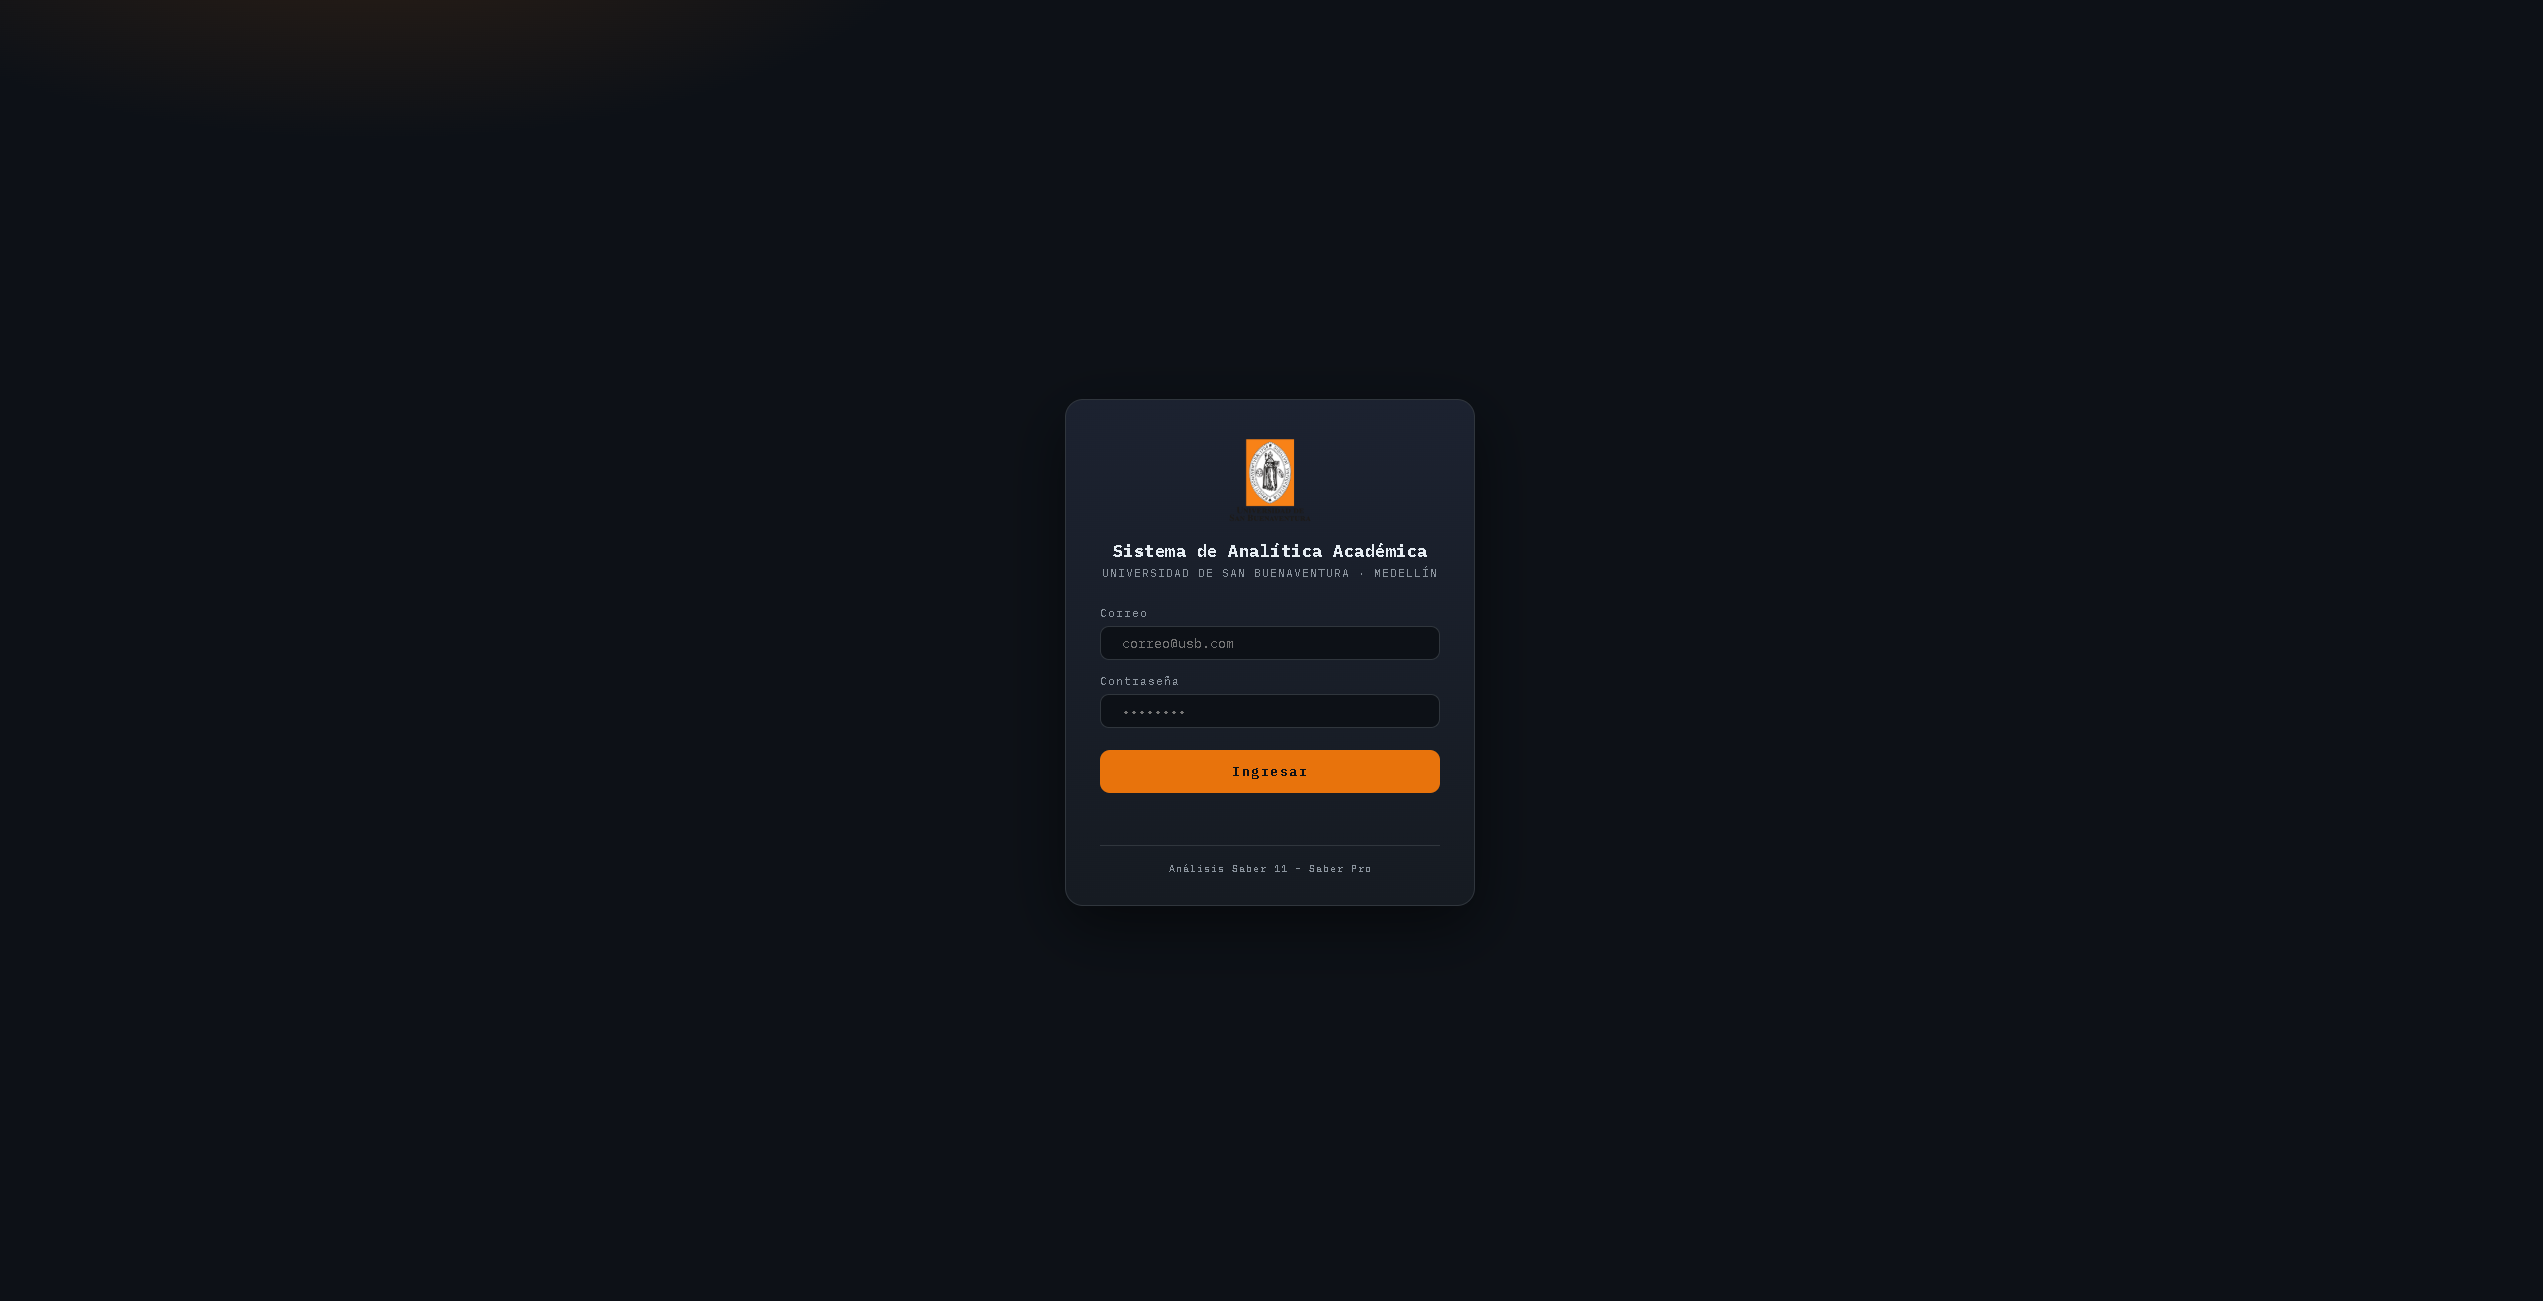
\includegraphics[width=0.7\textwidth]{images/login.png}
	\caption{Menú de login.}
	\label{fig:mi_imagen}
\end{figure}

\begin{figure}[h]
	\centering
	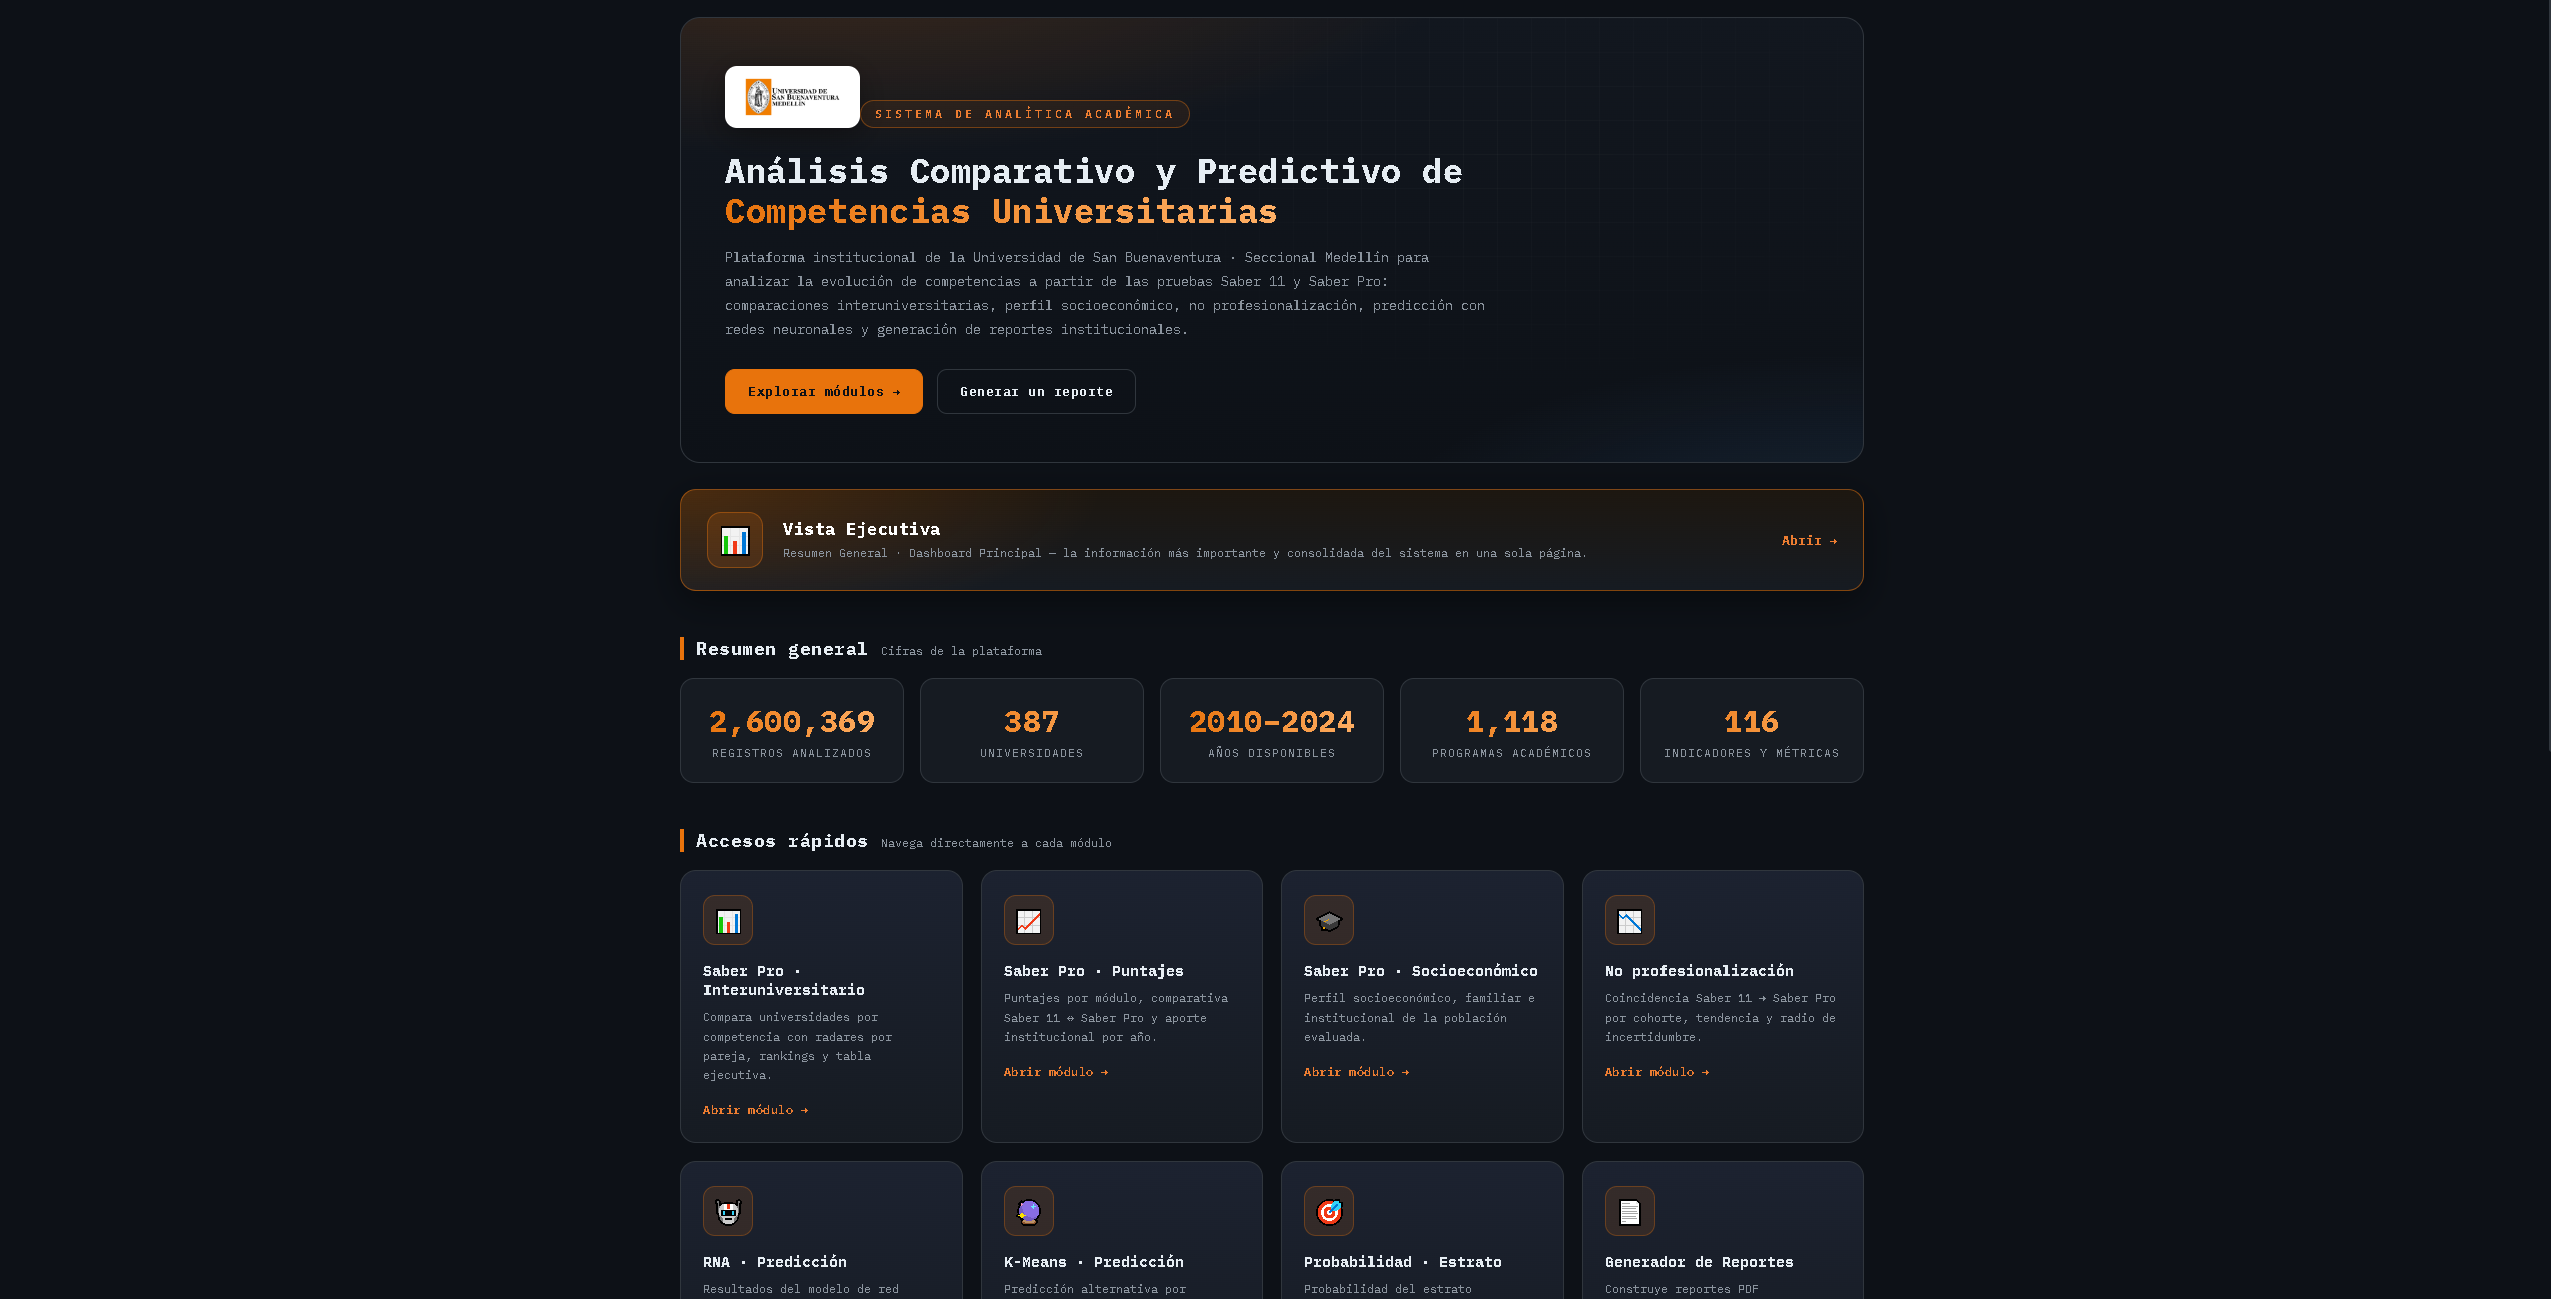
\includegraphics[width=0.7\textwidth]{images/home.png}
	\caption{Página de inicio.}
	\label{fig:mi_imagen}
\end{figure}

\begin{figure}[h]
	\centering
	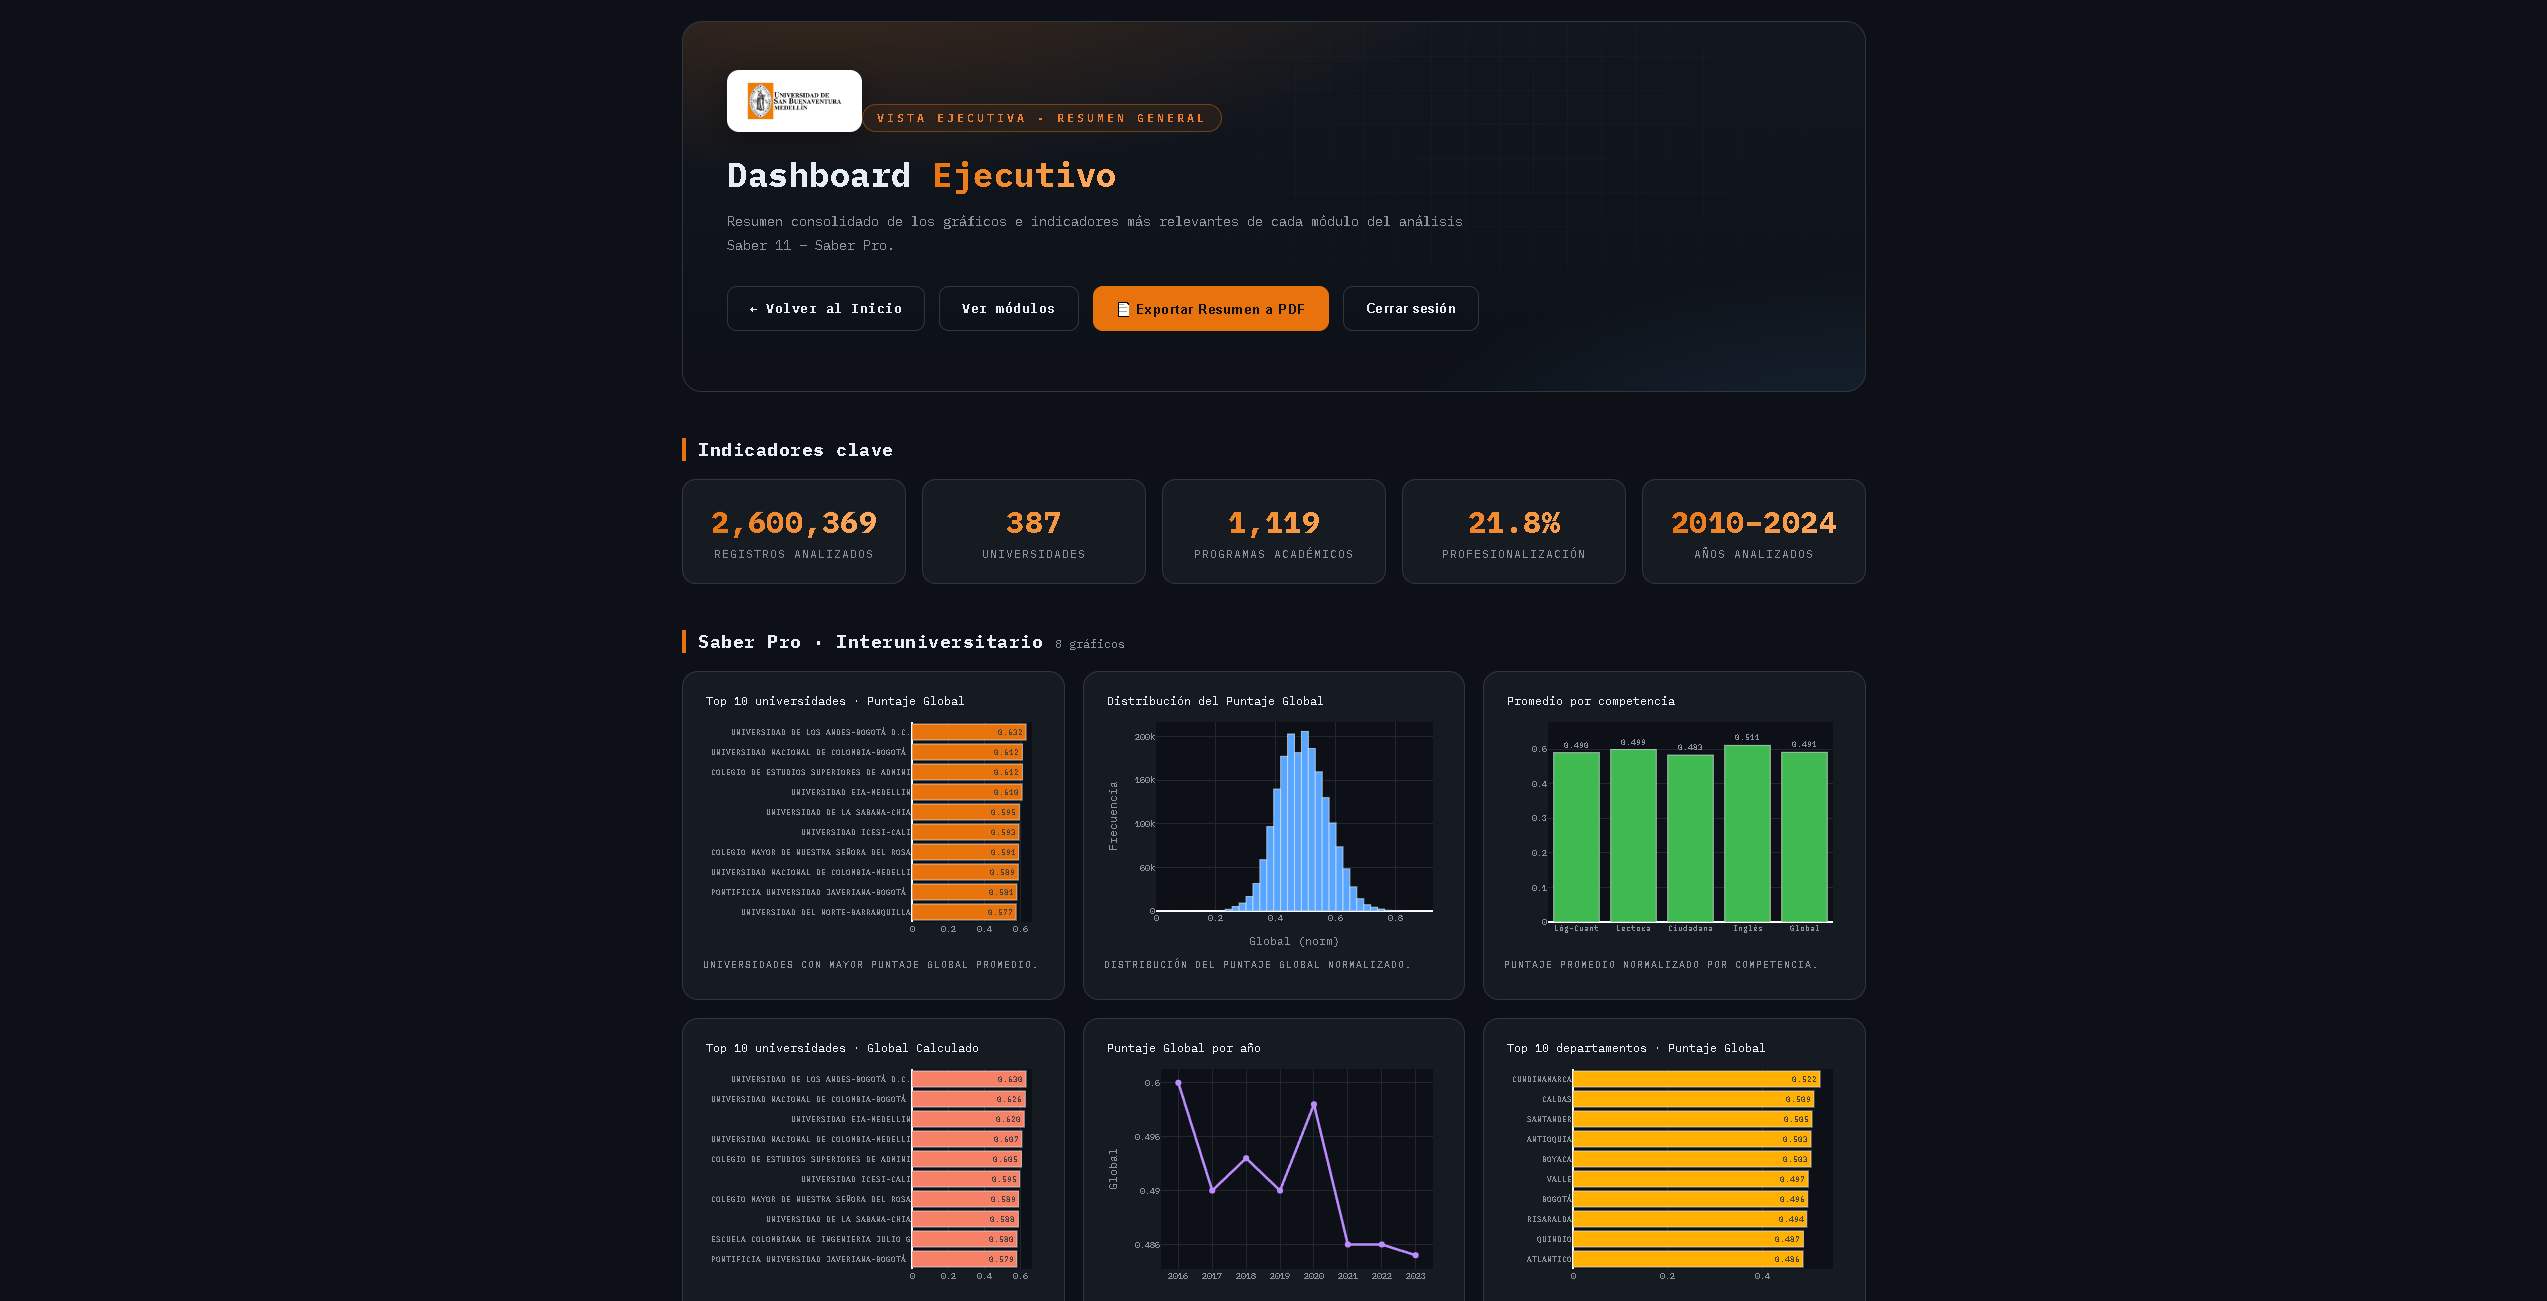
\includegraphics[width=0.7\textwidth]{images/vista_ejecutiva.png}
	\caption{Menú de resumen.}
	\label{fig:mi_imagen}
\end{figure}

\begin{figure}[h]
	\centering
	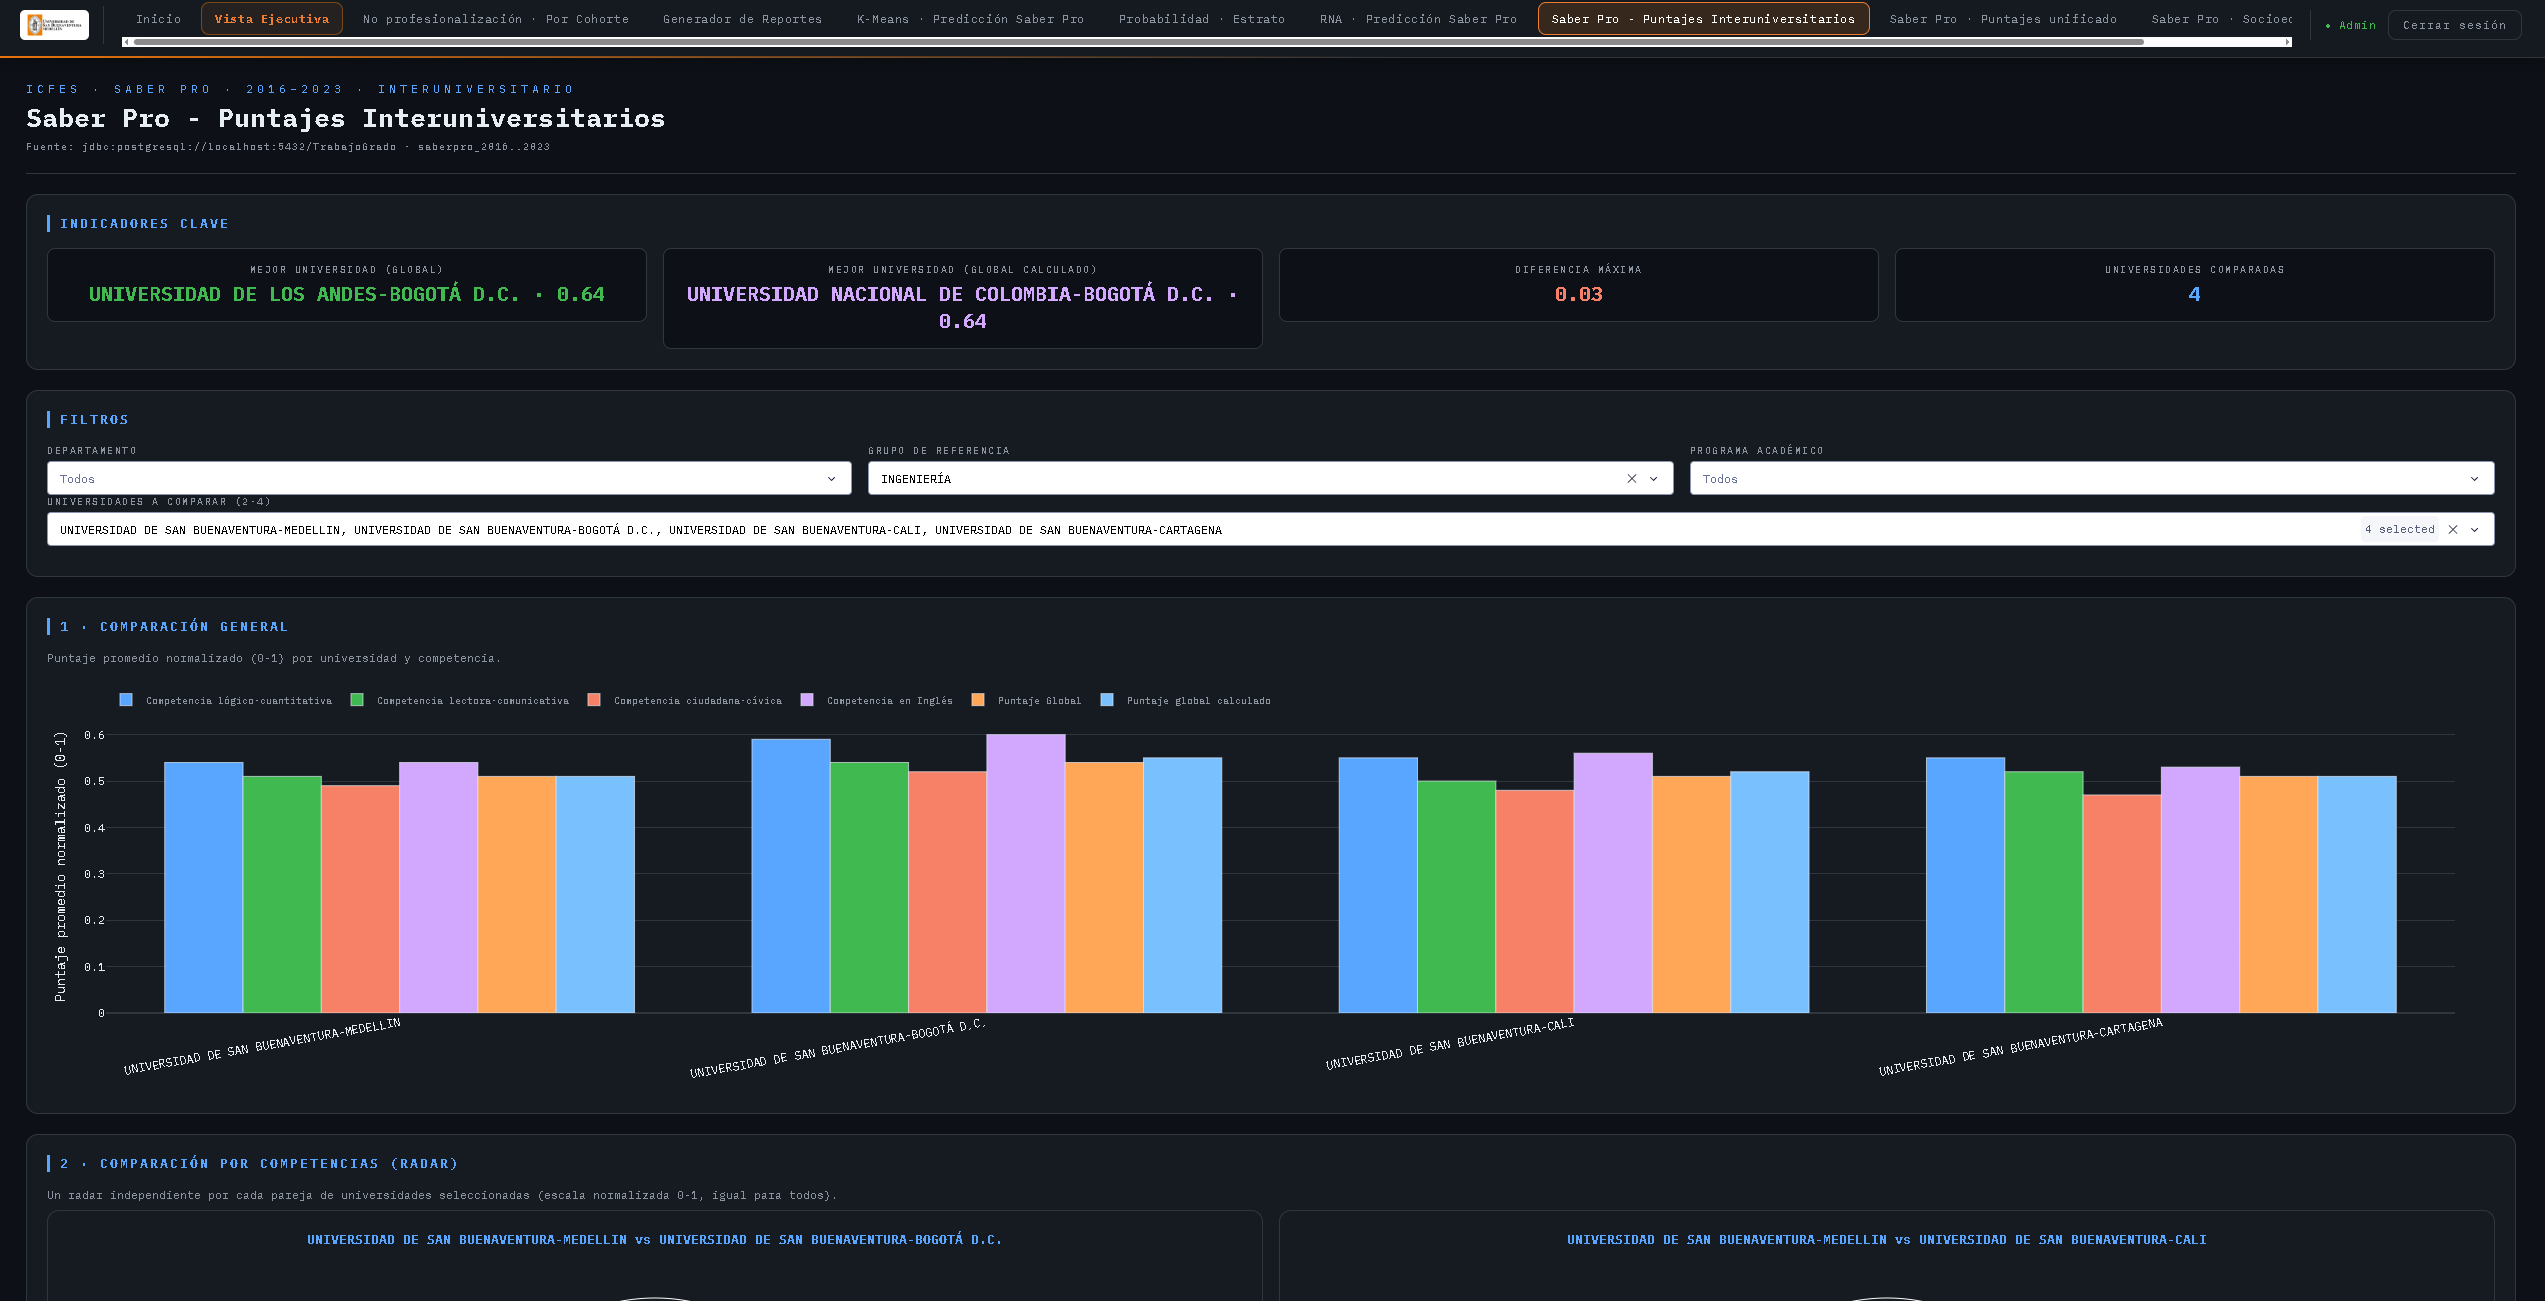
\includegraphics[width=0.7\textwidth]{images/puntajes_interuniv.png}
	\caption{Menú de comparativa para puntajes entre universidades.}
	\label{fig:mi_imagen}
\end{figure}

\begin{figure}[h]
	\centering
	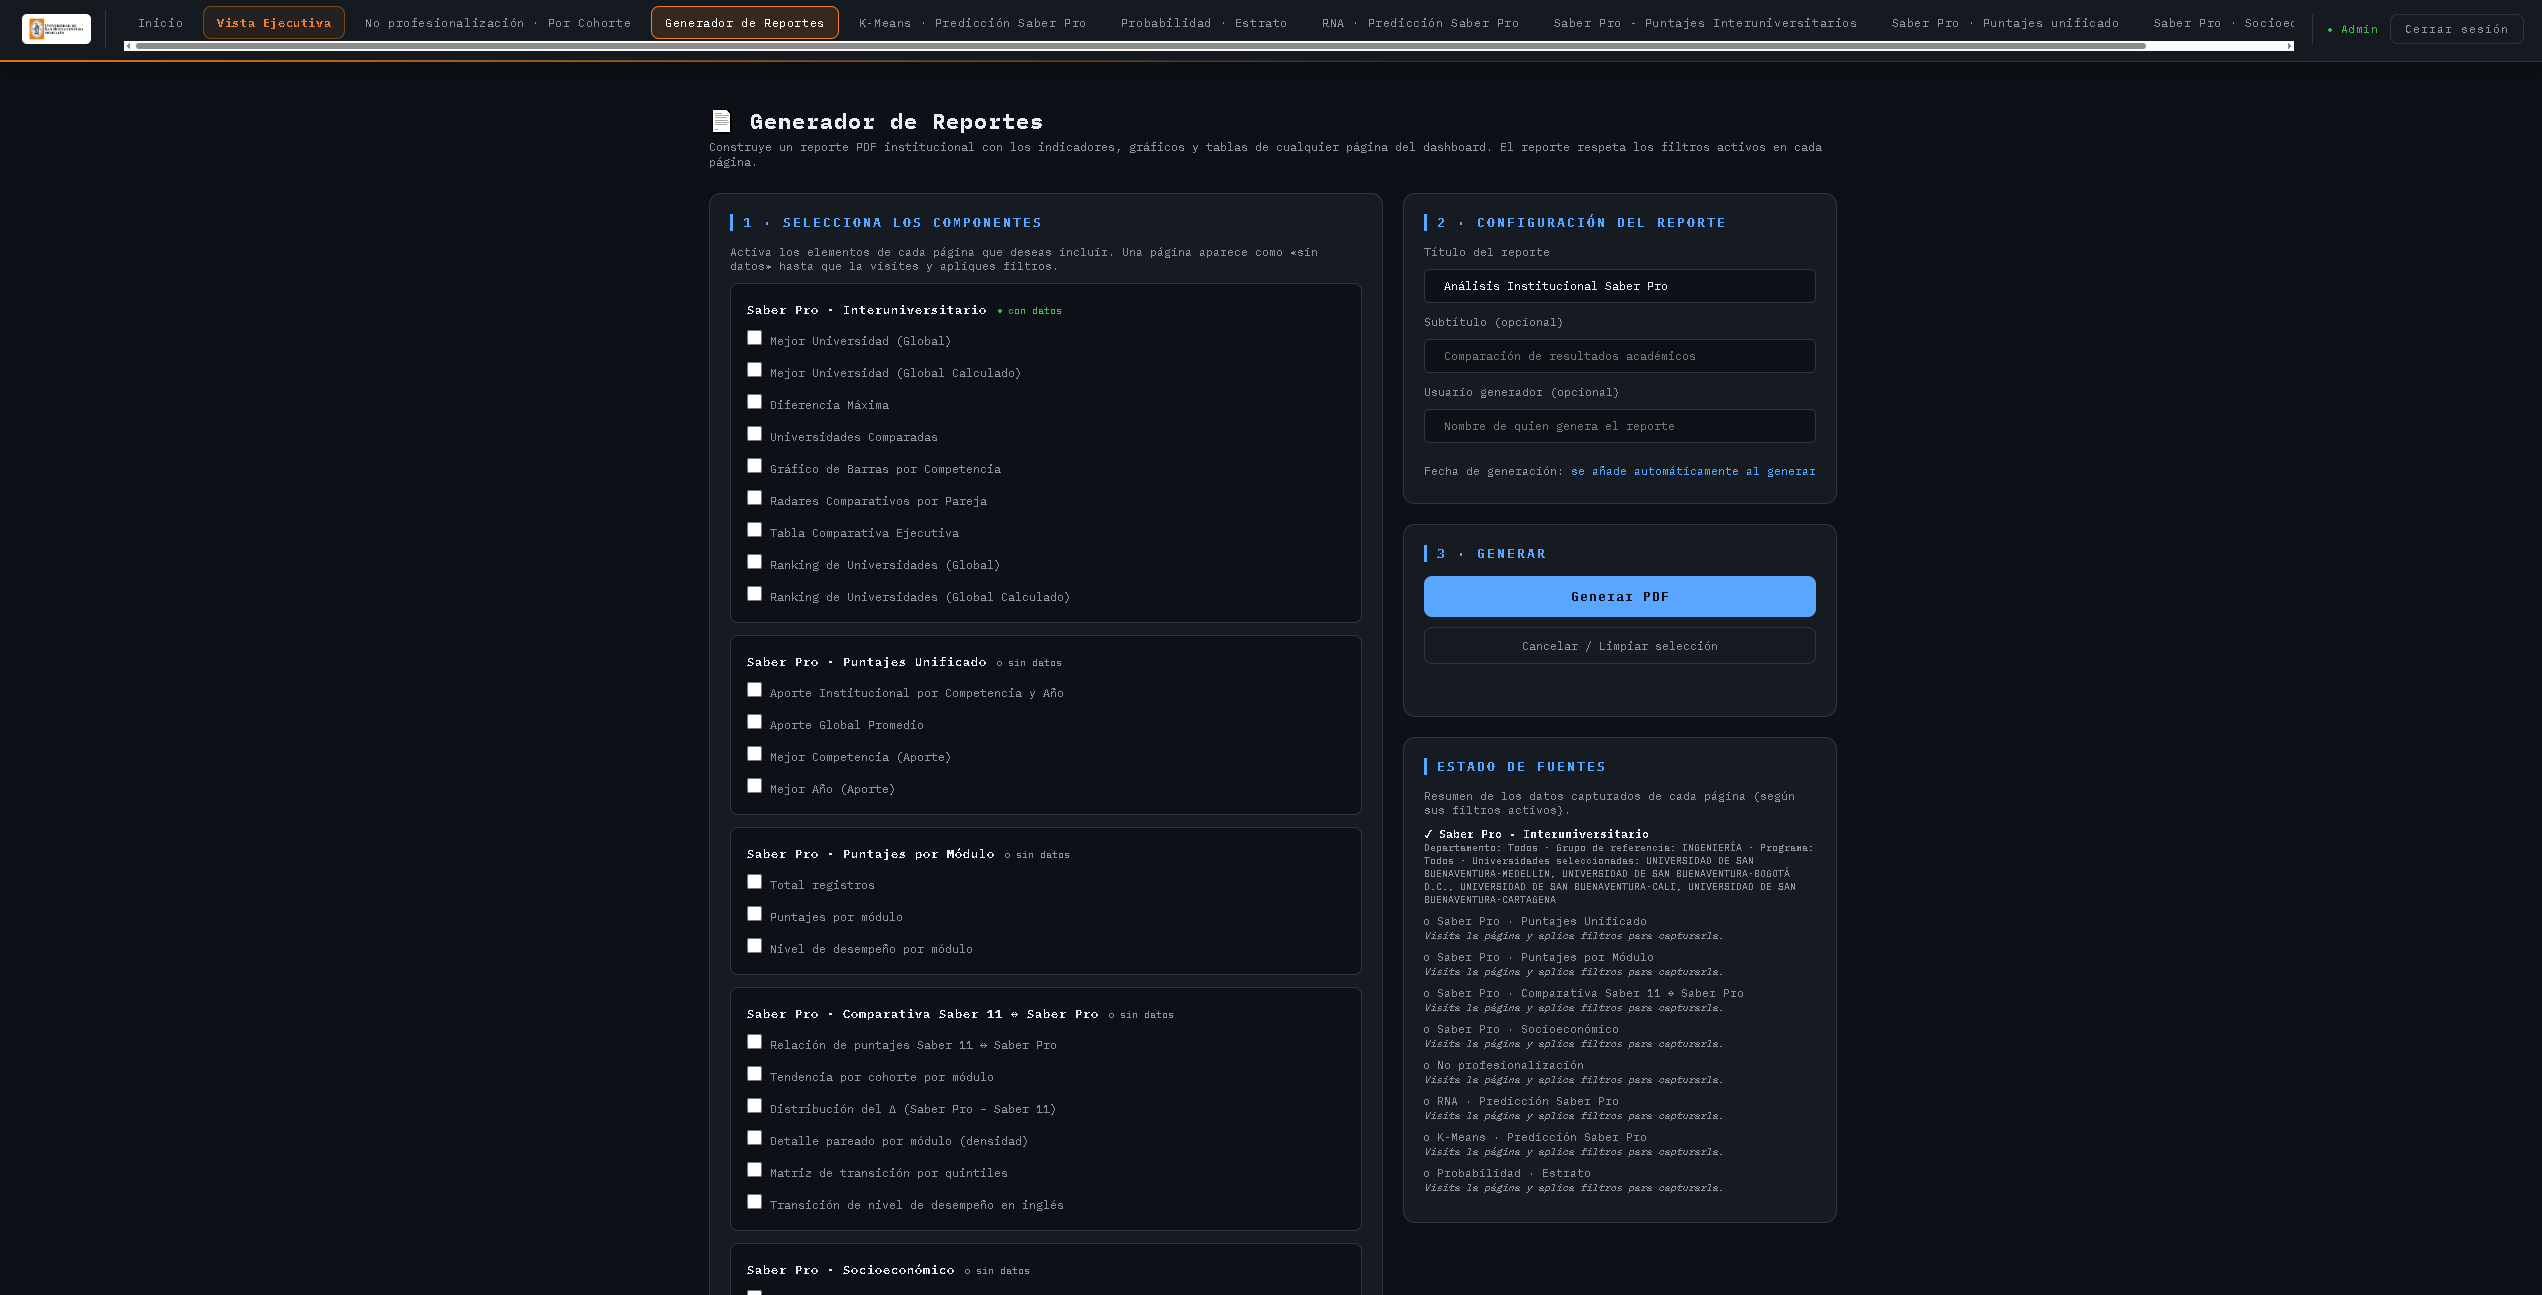
\includegraphics[width=0.7\textwidth]{images/generador_pdf.png}
	\caption{Menú para generar reportes en PDF.}
	\label{fig:mi_imagen}
\end{figure}

\begin{figure}[h]
	\centering
	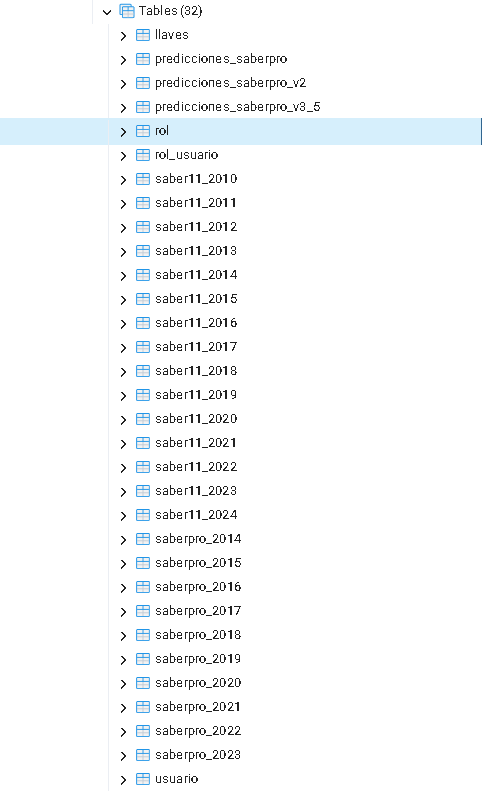
\includegraphics[width=0.7\textwidth]{images/database1.png}
	\caption{Tablas de la base de datos.}
	\label{fig:mi_imagen}
\end{figure}
	
	\cleardoublepage{}
	
	\selectlanguage{spanish}
	\section{REFERENCIAS}
	\begingroup
	\renewcommand{\section}[2]{}%
	\printbibliography[heading=none]
	\endgroup
	\selectlanguage{english}
	
\end{document}